\documentclass[12pt, a4paper]{report}
\usepackage{graphicx}
\usepackage{float}
\usepackage{booktabs}
\usepackage{caption}
\usepackage{rotating}
\usepackage{amsmath}
\usepackage [english]{babel}
\usepackage [autostyle, english = american]{csquotes}
\MakeOuterQuote{"}
\usepackage[margin=0.8in]{geometry}
\usepackage{hyperref}
\hypersetup{
     colorlinks   = true,
     citecolor    = gray
}
\usepackage{apacite}
\begin{document}

% THESIS COVER PAGE

% Choose Honors/Senior and Arts/Science below as appropriate.

\vspace*{0.1cm}
% LaTeX will remove blank space at the start or end of a page,
%   but the asterisk prevents this.

\centerline{\Large \textbf{Learning to Beat the Random Walk}}

\vspace*{12mm}

\centerline{\Large Using Machine Learning to Predict Changes in Exchange Rates}
\vspace*{12mm}
\centerline{\Large  A Senior Thesis}
\vspace*{5mm}
\centerline{\Large Presented to}
\vspace*{5mm}
\centerline{\Large The Faculty of the Economics Department of}
\vspace*{5mm}
\centerline{\Large Bates College}
\vspace*{5mm}

\begin{figure}[H]
    \centering
    
\includegraphics[scale=.15]{images/bates_logo.png}
\end{figure}

\vspace*{5mm}

\centerline{\Large In partial fulfillment of the requirements for the}

\vspace*{5mm}
\centerline{\Large Degree of Bachelor of Arts}

\vspace*{5mm}

\centerline{\Large by}

\vspace*{5mm}

\centerline{\Large Abdul Tawab Ajmal Safi}

\vspace*{5mm}

\centerline{\Large Lewiston, Maine}

\vspace*{5mm}

\centerline{\Large December 6, 2019}

\vspace*{16mm}

\centerline{\Large Advisor: Julieta Yung,Ph.D.}

\newpage



\vspace*{0.3cm}

{\LARGE \textbf{Abstract}\par}

\vspace*{6mm}
In my thesis, I use different machine learning techniques to predict the directional change in exchange rates. I start off by analyzing Uncovered Interest Rate Parity (UIP) and its failure to predict changes in exchange rates. Using linear regression, I show that the $\beta$ coefficient in UIP equation is not equal to zero over the short and long run. This shows the importance of currency risk premium for understanding changes in exchange rates. However, risk premium and market expectations are extremely difficult to measure. For this reason, Random Walk is the best model for predicting changes in the foreign exchange rates over the short run. This lead me to ask: \textbf{Can we use the latest machine learning techniques to predict foreign exchange rates more accurately than Random Walk model?} I explore various machine learning techniques including Principal Component Analysis (PCA), Support Vector Machines (SVM), Artificial Neural Networks (ANN), and Sentiment Analysis in an effort to predict the directional changes in exchange rates for a list of developed and developing countries.

\vspace*{3mm}

After exploring relevant literature on exchange rates, I analyze excess returns in the carry trade market by using historical exchange rate and interest rate data to create a simulation for trading on a monthly or semi-annual basis. I use the interest rate data of each country to sort them into portfolios for carry trade. The results show that investors can earn large profits over the short run by borrowing from low interest rate countries' bond market and investing in that of high interest rate countries. I also find that the returns on carry trade starts to reduce as the trading interval increases.

\vspace*{3mm}

According to the spanning hypothesis, the yield curve, its expectation and term premium component span all relevant information related to the economic performance of a country. This means that the economic situation of a country can be understood by analyzing its bond market. Based on the spanning hypothesis, I use Principal Component Analysis (PCA) to extract the level, slope, and curvature of the yield curve and its components. Then, taking the resultant principal components, I use Support Vector Machines (SVM) and Artificial Neural Networks (ANN) to predict the directional change in foreign exchange excess returns. Compared to the SVMs, the ANNs more accurately predict the directional change in the exchange rate excess returns over the short run. This difference is attributed to the ability of Artificial Neural Networks to learn abstract features from raw data.

\vspace*{3mm}

Finally, in the last chapter, I use sentiment analysis to evaluate the tonality of foreign exchange news articles from investing.com to develop a variable for understanding currency risk premium and market expectations in order to predict the directional changes in the exchange rates. In order to identify the model that most reliably captures the tonality of foreign exchange news articles, I use five different sentiment analysis models: Tonality model, VADER model, TextBlob model, Harvard IV-4 Dictionary model, and Loughran and Mcdonald Dictionary model. The results show that different sentiment models better predict the directional changes in exchange rates of different countries.

\vspace*{3mm}
Overall, this research finds evidence that machine learning models can more accurately predict directional change in exchange rates than the Random Walk model when the input features used to train the machine learning models are representative of the economic situation of a country. Hence, using macro-economic and financial theory to develop input features that capture the most relevant characteristics of a country's economy can help us understand short run movements in the foreign exchange markets.


\newpage

\vspace*{0.3cm}

{\LARGE \textbf{Acknowledgements}\par}

\vspace*{6mm}

I would like to thank Professor Yung for encouraging me to explore and develop different ideas throughout my thesis process. I would also like to thank Francesca for reminding me to sleep, motivating me to keep working hard, and being there for me throughout the semester. Thank you Will, for helping me edit my thesis and giving me advice how to better structure my sentences. Thank you Aktan, for pulling all nighters with me. Thank you Ghasharib and Kush for playing Catan with me to destress. Finally, I would like to thank my parents for all their effort and hard work that has allowed me to pursue my dreams.
\newpage

\tableofcontents

\chapter{Background}
\textbf{Exchange rate} refers to the value of one currency in terms of another i.e. how much of one currency can we buy with one unit of another currency. The exchange rate of a country \textbf{appreciates} when the value of its currency increases in terms of another currency. On the other hand, a currency \textbf{depreciates} when its value decreases in terms of another currency. Globalization has led economics to be more interconnected than ever before, making exchange rates important for both businesses and policy makers. Exchange rates are an important component of international trade which greatly influences the economic performance of a country. It influences the price of a good in the international market. For example, the exchange rate appreciation of a currency makes a country's imports cheaper while making exports expensive. Higher prices, in terms of other currencies, might make a country less competitive in the international market leading to a decrease in the demand for its goods. This can have a negative impact on the Gross Domestic Product (GDP) and subsequently the standard of living of a country. Hence, it has became increasingly imperative for economists to understand and model exchange rates in order to make wise decisions while conducting international trade or developing economic policies.

\vspace*{4mm}

Like other financial variables, changes in exchange rates are very hard to predict over the short run. This is because they are dictated by changes in the expectations about future economic fundamentals rather than by changes in the current ones. \textbf{Economic fundamentals} are macro-economic variables that are hypothesized to explain changes in exchange rate movements e.g. trade balances, money supply, national income etc. The current value of a macro-variable might vary drastically from its expected value \cite{wang2008exchange}. This means that current economic fundamentals might have very little, if any, use in forecasting exchange rates between countries with almost similar inflation rates. This gives rise to the \textbf{exchange rate disconnect puzzle}, which states that a random walk model does a better job at forecasting exchange rates over the short run than a model based on macro-economic fundamentals. A \textbf{random walk model} or a \textbf{naive model} is one that predicts the current value of a variable as its future value. It is difficult to beat the random walk model because exchange rates are more volatile than any of the candidate macro-economic fundamentals that we have. Another reason for the inefficiency of macro economic fundamentals in forecasting exchange rates is that their volatility remains similar across countries, whereas the volatility of exchange rates varies across different currency pairs. Finally, the exchange rate disconnect puzzle exists because currency volatility changes across fixed and floating regimes while the volatility of fundamentals does not \cite{meese1983empirical}.


\vspace*{4mm}

Trading on the foreign exchange market gave rise to the theory of \textbf{interest rate parity}, which states that return on investment in domestic bond market and foreign bond market should be the same. This assumes perfect competition and no arbitrage opportunity as positive returns on interest rate differential between countries is cancelled off by changes in the exchange rate. This leads to the idea of \textbf{uncovered interest rate parity (UIP)}, which states that domestic interest rate should be equal to foreign interest rate plus expected change in exchange rates. According to Aggarwal (2013), "If investors are risk-neutral and have rational expectations, the future exchange rate should perfectly adjust given the present interest-rate differential." This means that the expected change in exchange rate over a certain period is equal to that period's risk-free interest rate differential between the foreign and domestic bond market \cite{aggarwal2013uncovered}. Following is the equation for UIP:

\[E_t[s_{t+1}] - s_t= i_t - i_t^*

In the equation above, $\[E_t[s_{t+1}] - s_t$ indicates the change in exchange rate from one period to another. We use $i_t$ to show domestic interest rate and $i_t^*$ to show foreign interest rate. The subscript \textbf{t} indicates the current time period, while the subscript \textbf{t+1} indicates one period future time period. The equation above can be further simplified into the following equation:

\[\Delta s_{t+1}= i_t - i_t^*

In the equation above, $\Delta s_{t+1}$ indicates the change in exchange rate from one period to another. According to the equation, if the domestic interest rate $i_t$ is greater than the foreign interest rate $i_t^*$ then the domestic currency will be expected to depreciate for interest rate parity to hold. However, this theory does not hold in reality.

\vspace*{4mm}

Exchange rate changes are not compensated by interest rate differentials. "If anything, the opposite holds true empirically - high-interest-rate currencies tend to appreciate while low-interest-rate currencies tend to depreciate. As a consequence, carry trades form a portfolio investment strategy, violate the uncovered interest parity and give rise to the 'forward premium puzzle'" \cite{menkhoff2011risk}. \textbf{Carry Trade} is the most popular investment strategy in the foreign exchange market. According to it, we can earn a profit by borrowing from countries with low interest rate and investing in countries with high interest rate. The success of carry trade indicates the failure of UIP which gives rise to the forward premium puzzle or the "Fama Puzzle". According to it, if the domestic interest rate is greater than the foreign interest rate it causes the domestic currency to appreciate instead of depreciate, which is contrary to what theory suggests \cite{fama1984forward}. A theoretically convincing and straight forward solution for this puzzle is the consideration of the time-varying risk premium. \textbf{Risk Premium} or \textbf{Risk Premia} is the compensation that risk averse investors require for holding assets denominated in foreign currencies. Investors in the foreign exchange market are always exposed to currency risk, which is the risk that the value of foreign currency might change leading to loss. A positive risk premium shows that the investors view a certain foreign currency as risky asset, while a negative risk premium shows that the investors view a certain currency as a safe asset. It is the inclusion of the time varying risk premium component in the UIP equation that might help us explain the Fama Puzzle i.e. the negative correlation between ex post depreciation and the interest rate differentials.

\[\Delta s_{t+1}= i_t - i_t^* + RP_t

In the equation above, the $RP_t$ indicates the time varying risk premium of the currency market. According to the "New Fama Puzzle", it is not only the risk premium but also the not unbiasedness of the expectation of exchange rate changes that causes the failure of UIP. Accounting for risk premia alone does not entirely cause the UIP to be true. Hence it will be important to integrate an expectation variable extracted from surveys or news paper analysis into our model in order to be consistent with economic theory \cite{bussiere2018new}.

\chapter{Testing for UIP}
\section{Regression Analysis}
In this section, I am going to test for uncovered interest rate parity by using a univariate OLS regression model. I am going to use monthly change in US dollars in terms of British Pounds (GBP) as the dependent variable. United States is considered as the domestic country while United Kingdoms is considered as the foreign country in the model. The dataset consists of monthly data from 1999 to 2019. The model used to test for UIP is adopted from \cite{hansen1980forward}.

\[\Delta s_{t+n}= \alpha + \beta(i_t - i_t^*) + e_{t+n}

In the equation above, $\Delta s_{t+n}$ indicates the change in exchange rate \textbf{n} periods ahead. $\alpha$ is the value of the constant or intercept in the model. $e_{t+n}$ shows the time varying error term of the model. All the residuals of the model are stored in the error term. $i_t - i_t^*$ indicates the interest rate differential between the domestic and foreign country i.e. US and UK respectively. $\beta$ shows the regression coefficient of the interest rate differential. It indicates how much GBP/USD will move based on one unit change in the interest rate differential. In order for UIP to hold, $\alpha $ should be equal to zero and $\beta$ should be equal to 1. A $\beta$ value of positive one indicates that the interest rate differential is positively correlated with change in exchange rate. An $\alpha$ value of zero indicates that there is no constant in the model i.e. all movements in the exchange rate are explained by changes in the interest rate differential.

\vspace*{4mm}

One might hypothesize that changes in the interest rate differential might take time to influence changes in exchange rates. This means that the UIP might not hold over the short run but it might hold over the long run. In order to test for this hypothesis, I developed three different regression models at varying lagged intervals. The first model checks for the existence of UIP over the very short run as it regresses changes in current exchange rate on current interest rate differential. The second model checks for UIP over a 6 month period by checking the efficiency of the current interest rate differential in predicting changes in the 6 month ahead exchange rate. Lastly, the final model check for UIP over the long run, by checking the efficiency of current interest rate differential in predicting changes in one year ahead exchange rates. According to theory, UIP does not hold over the short or long run. The $\beta$ coefficient over the short run will be less than 0 indicating the existence of risk premium, while it might become positive over the long run (but it never equals 1).

\vspace*{4mm}

\subsection{Results}
\subsubsection{\hfil UIP Test over Zero Lagged Interval \hfil}

\vspace*{5mm}

\begin{center}
\begin{tabular}{lclc}
\toprule
\textbf{Dep. Variable:}    &     GBP/USD      & \textbf{  R-squared:         } &     0.051   \\
\textbf{Model:}            &       OLS        & \textbf{  Adj. R-squared:    } &     0.048   \\
\textbf{Method:}           &  Least Squares   & \textbf{  F-statistic:       } &     13.19   \\
\textbf{Date:}             & Fri, 29 Nov 2019 & \textbf{  Prob (F-statistic):} &  0.000343   \\
\textbf{Time:}             &     19:13:35     & \textbf{  Log-Likelihood:    } &    603.14   \\
\textbf{No. Observations:} &         245      & \textbf{  AIC:               } &    -1202.   \\
\textbf{Df Residuals:}     &         243      & \textbf{  BIC:               } &    -1195.   \\
\textbf{Df Model:}         &           1      & \textbf{                     } &             \\
\bottomrule
\end{tabular}
\begin{tabular}{lcccccc}
                   & \textbf{coef} & \textbf{std err} & \textbf{t} & \textbf{P$>$$|$t$|$} & \textbf{[0.025} & \textbf{0.975]}  \\
\midrule
\textbf{Intercept} &       0.0020  &        0.001     &     1.491  &         0.137        &       -0.001    &        0.005     \\
\textbf{x}         &      -0.0040  &        0.001     &    -3.632  &         0.000        &       -0.006    &       -0.002     \\
\bottomrule
\end{tabular}
\begin{tabular}{lclc}
\textbf{Omnibus:}       & 19.218 & \textbf{  Durbin-Watson:     } &    1.598  \\
\textbf{Prob(Omnibus):} &  0.000 & \textbf{  Jarque-Bera (JB):  } &   31.069  \\
\textbf{Skew:}          &  0.474 & \textbf{  Prob(JB):          } & 1.79e-07  \\
\textbf{Kurtosis:}      &  4.465 & \textbf{  Cond. No.          } &     1.32  \\
\bottomrule
\end{tabular}
%\caption{OLS Regression Results}
\end{center}

\begin{figure}[H]
    \centering
    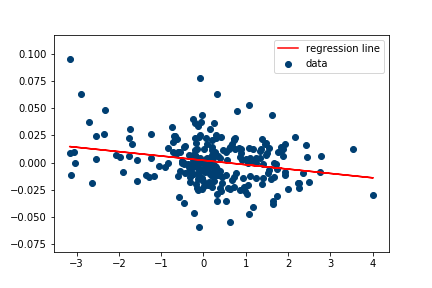
\includegraphics[scale=.85]{images/reg/current.png}
    \caption{Current change in exchange rate against current interest rate differential}
    \label{simulationfigure}
\end{figure}

According to the regression results and figure above, the UIP does not hold over the zero lagged interval. The $\beta$ coefficient for the interest rate differential has a value of -0.0040 which is as per the Fama puzzle and it validates the presence of the risk premium component. The $\beta$ coefficient is statistically significant at 99\% significance level. The intercept $\alpha$ is also not equal to zero. The scatterplot above shows that the interest rate differential is negatively correlated with the change in exchange rate which violates UIP. The results indicate that UIP does not hold over the very short run.





\subsubsection{\hfil UIP Test over 6 Month Lagged Interval \hfil}

\vspace*{5mm}

\begin{center}
\begin{tabular}{lclc}
\toprule
\textbf{Dep. Variable:}    &      GBP/USD     & \textbf{  R-squared:         } &     0.026   \\
\textbf{Model:}            &       OLS        & \textbf{  Adj. R-squared:    } &     0.022   \\
\textbf{Method:}           &  Least Squares   & \textbf{  F-statistic:       } &     6.442   \\
\textbf{Date:}             & Fri, 29 Nov 2019 & \textbf{  Prob (F-statistic):} &   0.0118    \\
\textbf{Time:}             &     19:45:23     & \textbf{  Log-Likelihood:    } &    607.42   \\
\textbf{No. Observations:} &         248      & \textbf{  AIC:               } &    -1211.   \\
\textbf{Df Residuals:}     &         246      & \textbf{  BIC:               } &    -1204.   \\
\textbf{Df Model:}         &           1      & \textbf{                     } &             \\
\bottomrule
\end{tabular}
\begin{tabular}{lcccccc}
                   & \textbf{coef} & \textbf{std err} & \textbf{t} & \textbf{P$>$$|$t$|$} & \textbf{[0.025} & \textbf{0.975]}  \\
\midrule
\textbf{Intercept} &       0.0018  &        0.001     &     1.357  &         0.176        &       -0.001    &        0.005     \\
\textbf{x}         &      -0.0028  &        0.001     &    -2.538  &         0.012        &       -0.005    &       -0.001     \\
\bottomrule
\end{tabular}
\begin{tabular}{lclc}
\textbf{Omnibus:}       & 17.308 & \textbf{  Durbin-Watson:     } &    1.545  \\
\textbf{Prob(Omnibus):} &  0.000 & \textbf{  Jarque-Bera (JB):  } &   29.657  \\
\textbf{Skew:}          &  0.403 & \textbf{  Prob(JB):          } & 3.63e-07  \\
\textbf{Kurtosis:}      &  4.490 & \textbf{  Cond. No.          } &     1.32  \\
\bottomrule
\end{tabular}
%\caption{OLS Regression Results}
\end{center}

\begin{figure}[H]
    \centering
    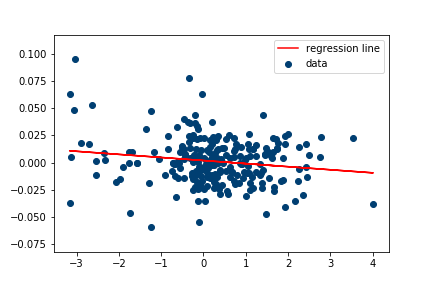
\includegraphics[scale=.85]{images/reg/current_six.png}
    \caption{6-month-ahead change in exchange rate against current interest rate differential}
    \label{simulationfigure}
\end{figure}

According to the regression results and figure above, the UIP does not hold over the six month lagged interval. The $\beta$ coefficient for the interest rate differential has a value of -0.0028 which is as per the Fama puzzle and it validates the presence of the risk premium component. The $\beta$ coefficient is statistically significant at 95\% significance level. The $\beta$ coefficient has been reduced in magnitude and significance compared to the zero lagged regression results. The intercept $\alpha$ is also not equal to zero. The scatterplot above shows that the interest rate differential is negatively correlated with the change in exchange rate which violates UIP. The results indicate that UIP does not hold over the over six month lagged interval.

\newpage

\subsubsection{\hfil UIP Test over 1 Year Lagged Interval \hfil}

\vspace*{5mm}

\begin{center}
\begin{tabular}{lclc}
\toprule
\textbf{Dep. Variable:}    &        GBP/USD   & \textbf{  R-squared:         } &     0.003   \\
\textbf{Model:}            &       OLS        & \textbf{  Adj. R-squared:    } &    -0.001   \\
\textbf{Method:}           &  Least Squares   & \textbf{  F-statistic:       } &    0.6652   \\
\textbf{Date:}             & Fri, 29 Nov 2019 & \textbf{  Prob (F-statistic):} &    0.416    \\
\textbf{Time:}             &     20:23:40     & \textbf{  Log-Likelihood:    } &    604.55   \\
\textbf{No. Observations:} &         248      & \textbf{  AIC:               } &    -1205.   \\
\textbf{Df Residuals:}     &         246      & \textbf{  BIC:               } &    -1198.   \\
\textbf{Df Model:}         &           1      & \textbf{                     } &             \\
\bottomrule
\end{tabular}
\begin{tabular}{lcccccc}
                   & \textbf{coef} & \textbf{std err} & \textbf{t} & \textbf{P$>$$|$t$|$} & \textbf{[0.025} & \textbf{0.975]}  \\
\midrule
\textbf{Intercept} &       0.0013  &        0.001     &     0.980  &         0.328        &       -0.001    &        0.004     \\
\textbf{x}         &      -0.0009  &        0.001     &    -0.816  &         0.416        &       -0.003    &        0.001     \\
\bottomrule
\end{tabular}
\begin{tabular}{lclc}
\textbf{Omnibus:}       & 25.499 & \textbf{  Durbin-Watson:     } &    1.511  \\
\textbf{Prob(Omnibus):} &  0.000 & \textbf{  Jarque-Bera (JB):  } &   49.022  \\
\textbf{Skew:}          &  0.544 & \textbf{  Prob(JB):          } & 2.26e-11  \\
\textbf{Kurtosis:}      &  4.887 & \textbf{  Cond. No.          } &     1.26  \\
\bottomrule
\end{tabular}
%\caption{OLS Regression Results}
\end{center}

\begin{figure}[H]
    \centering
    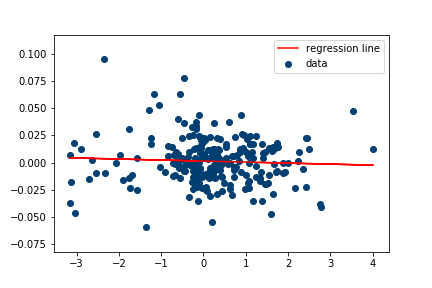
\includegraphics[scale=.85]{images/reg/current_12.png}
    \caption{1-year-ahead change in exchange rate against current interest rate differential}
    \label{simulationfigure}
\end{figure}

According to the regression results and figure above, the UIP does not hold over the one year lagged interval. The $\beta$ coefficient for the interest rate differential has a statistically insignificant value of value of -0.0009. This means that there is a possibility that the regression coefficient is positive instead of negative. This shows that the existence of the Fama puzzle is not certain over the long run i.e. the current risk premium component has little, if any, influence on 1 year ahead exchange rate. The intercept $\alpha$ is also not equal to zero. The scatterplot above shows that the interest rate differential is still slightly negatively correlated with the change in exchange rate which violates UIP. The results indicate that UIP also does not hold over a 1 year lagged interval.

\newpage

\subsection{Discussion}
As the theory suggests, the uncovered interest rate parity (UIP) does not hold over the short and long run. Our regression results show that the $\beta$ coefficient and intercept $\alpha$ at all three lagged intervals were not equal to 1 and 0 respectively. This means that the UIP did not hold true at any time interval within 1 year for the GBP/USD currency pair. Over the zero and six month lagged interval, the forward premium puzzle seemed to exist that the $\beta$ coefficient was negative and statistically significant. This means that the current currency risk premium can influence changes in six month ahead exchange rates. This, however, does not appear to be the case for the one year lagged interval, as the $\beta$ coefficient was still negative but statistically insignificant. This indicates that there is a possibility that the $\beta$ coefficient might be positive. These results show that the influence of the current currency risk premium on the exchange rate starts to depreciate over time.

\section{Carry Trade Portfolio Simulation}
Carry trade is a popular currency trading strategy that invests in high interest currencies by borrowing from low interest currencies. "Carry trade is at the core of active currency management and is designed to exploit deviations from uncovered interest rate parity (UIP). If UIP holds, the interest rate differential is an average offset by a commensurate depreciation of the investment currency and the expected carry trade return is equal to zero" \cite{cenedese2014foreign}. This means that the popularity of carry trade and the existence of excess returns in it indicates the existence of the Fama Puzzle. In order for UIP to hold there should be no arbitrage opportunity in the economy which means that carry trade should not be profitable. This, however, is never the case. In  this section, I am going to use basic carry trade strategy to prove that UIP does not hold.

\vspace*{4mm}

Carry trade, in the past, has delivered considerable excess returns and a sharpe ratio of more than twice that of the US stock market. This has made it into the most popular trading strategy in the currency market. However, according to the current literature high profits in carry trade are no free lunch in the sense that they act as compensation for investors for bearing risk \cite{cenedese2014foreign}. The returns from carry trade compensate investors for exposure to systematic risk that might lead to large future carry trade losses during periods of high market variance. Interest rate measures the level of the risk in an economy. High interest rates indicate risky currencies that pay the largest premium, while low interest rate currencies are less risky and offer insurance against aggregate risk. The returns for high interest rate currencies tend to fall during periods of high economic uncertainty whereas the returns for low interest rate currencies tend to rise \cite{berg2018measures}. It is this behavior of the currency risk premium component that explains the forward premium puzzle and the excess returns it causes in carry trade.

\vspace*{4mm}

"While the average carry trade is profitable, the performance of the individual carry trade varies across currencies, with trades against the Swiss Franc earning a low 0.6\% annual excess return, and trade against the Danish Krone earning a high 9.3\% annual excess return" \cite{burnside2011carry}. Individual currency trading has higher exposure to risk and uncertainty because it relies on the economic conditions of only one specific country. According to financial trading, diversifying an investment portfolio always yields better results than investing in an individual asset. For this reason, I am going to explore different weighted carry trade portfolios using a diverse set of developed and developing countries. The countries being considered for the analysis are Australia, Canada, China, Chile, Czech Republic, Colombia, Hungary, Indonesia, Japan, Mexico, Norway, New Zealand, Poland, South Africa, Singapore, Sweden, Switzerland, United Kingdoms, and Brazil. All countries exchange rates are calculated with USD as its base value. This is done to calculate the profit a US investor will make by participating in carry trade.

\vspace*{4mm}

Excess return in carry trade is the product of the amount of investment with the interest rate differential between the low and high interest rate currencies while accounting for the change in exchange rates. Transaction cost is another additional expense that needs to be accounted for while calculating returns on carry trade. In our analysis, for simplicity purposes, I am going to assume our transaction cost to be zero. Percentage return on carry trade varies based on the trading interval used. Trading on the currency market can be done on daily, weekly, monthly, quarterly, semi-annually, or annual intervals. Craig Burnside (2011)'s carry trade portfolio strategy earned an average annual profit of 6\% with a standard deviation of 9.5\%. In my analysis, I am going to use monthly and semi-annual trading basis. Using a monthly trading strategy means that during the start of every month currencies are sorted as per their interest rate. Afterwards, a portfolio is constructed shorting the lowest interest rate currencies and going long on the highest interest rate currencies. By the end of every month excess returns are calculated for the carry trade. A similar procedure with 6 month lagged intervals are used for the semi-annual trading strategy. The formula for calculating the payoff to carry trade strategy is taken from Craig Burnside (2011):

\[z_{t+n}= (1+i_t^*)\frac{s_{t+n}}{s_t} - (1+i_t)

In the above equation, $z_{t+n}$ shows the payoff for investing one USD in carry trade. $i_t^*$ represents the interest rate of the country that we are investing in, while $i_t$ represents the interest rate of the country we are borrowing from. $\frac{s_{t+1}}{s_t}$ represents the change in exchange rate over \textbf{n} period of time.

\vspace*{4mm}

The dataset used for carry trade analysis consists of monthly treasury bills and exchange rate data ranging from 1999 to 2018. Treasury bills with one month bond maturity are used as a proxy for interest rate of different countries. Higher bond maturities are not used because the average excess return declines to zero as the maturity increases. This means that carry trade strategy implemented with treasury bills is more profitable than that implemented on long term bonds \cite{lustig2013term}. The carry trade model equips a rolling one month horizon investment strategy. This means that no train or test dataset is required for the development of the model. The model uses basic carry trade strategy, which invests in high interest currencies and borrows from low interest rate currencies, in combination with a weighting mechanism to construct portfolios. Weights are manual assigned by a trader at the beginning of the trading interval. A weight of "100\%" would mean that the model should borrow 100\% of the investment amount from the country with lowest interest rate and invest all of it in the country with the highest interest rate. Similarly, a weight of "60\% and 40\%" means that the model should borrow 60\% from the country with lowest interest rate and 40\% from the country with the second lowest interest rate and then invest 60\% in the country with the highest interest rate and 40\% in the country with the second highest interest rate. In the next section, results for different weights at varying trading intervals are presented.

\newpage

\subsection{Results}
\vspace*{4mm}
\subsubsection{\hfil Excess Return of Single Currency Portfolio on Monthly Basis\hfil}
\vspace*{-8mm}
\begin{figure}[H]
    \centering
    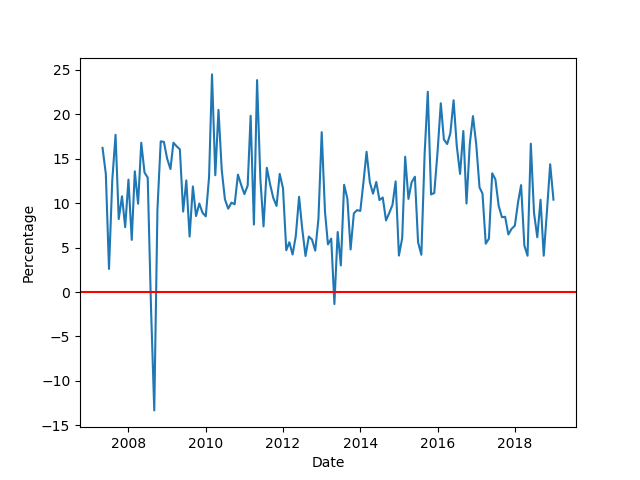
\includegraphics[scale=.98]{images/carryTrade/monthly1.png}
    \caption{Percentage Profit From Monthly Carry Trade (Weight = [100])}
    \label{simulationfigure}
\end{figure}

\vspace*{5mm}

According to the single currency carry trade portfolio strategy, every month 100\% the amount of investment is borrowed from the country with the lowest interest rate and invested in the country with the highest interest rate. Every month the borrowing and investing country changes based on the global changes in interest rate. The average monthly percentage profit for a single currency carry trade portfolio strategy is 10.89\%. Single currency trading is extremely profitable but volatile and risky at the same time. It can lead to huge profits or huge losses based on the economic situation of a country. As we can see the strategy makes its biggest loss around 2008, which was during the financial crisis. However, the biggest loss of the strategy is about 10\% point smaller than the biggest profit. Diversifying our portfolio by including more currencies might be a good idea to minimize loss during times of uncertainty such as the 2008 recession.

\newpage

\subsubsection{\hfil Excess Return of Multi-Currency Portfolio on Monthly Basis\hfil}
\vspace*{-8mm}
\begin{figure}[H]
    \centering
    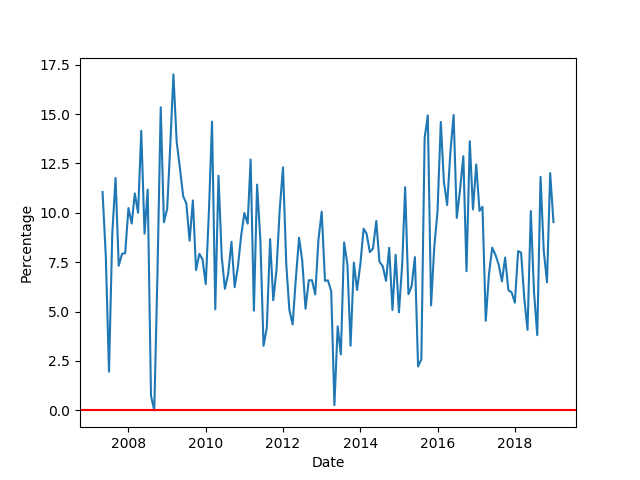
\includegraphics[scale=.98]{images/carryTrade/monthly2.png}
    \caption{Percentage Profit From Monthly Carry Trade (Weight = [40,30,30])}
    \label{simulationfigure}
\end{figure}

\vspace*{5mm}

According to the multi-currency carry trade portfolio strategy, every month the investment amount is borrowed from three countries with the lowest interest rate with 40\% , 30\% , and 30\% weight respectively. Afterwards the same weights are used to invest in the top three countries with the highest interest rate. Every month the borrowing and investing countries changes based on the global changes in interest rate. The average monthly percentage profit for a multi-currency carry trade portfolio strategy is 8.29\%. Although our average excess return reduced from the single currency carry trade portfolio, our strategy does not face any major losses. Diversifying our portfolio by borrowing from and lending to multiple countries has reduced our exposure to loss during times of high uncertainty. Our loss during 2008 recession from single currency portfolio strategy to a multi currency portfolio strategy fell from about 14\% to about 0\%. As supported by the theory, diversifying our portfolio leads to a reduction in our average profit and the possibility of loss.

\newpage

\subsubsection{\hfil Excess Return of Multi-Currency Portfolio on Semi-Annual Basis\hfil}
\vspace*{-8mm}
\begin{figure}[H]
    \centering
    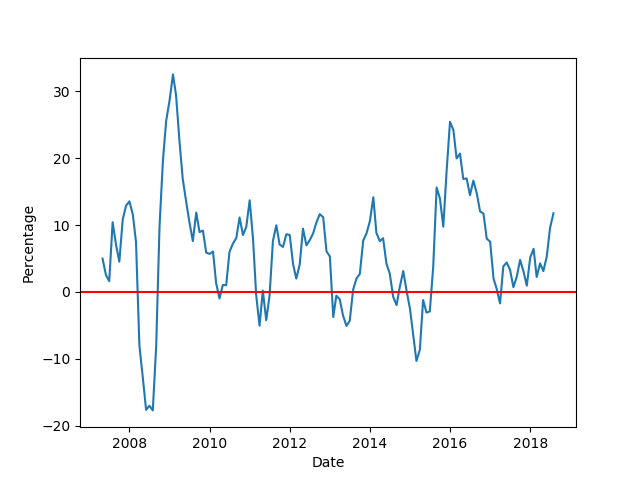
\includegraphics[scale=.98]{images/carryTrade/halfYear1.png}
    \caption{Percentage Profit From Semi-Annual Carry Trade (Weight = [40,30,30])}
    \label{simulationfigure}
\end{figure}

\vspace*{5mm}

According to the multi-currency carry trade portfolio strategy, every half a year the investment amount is borrowed from three countries with the lowest interest rate with 40\% , 30\% , and 30\% weight respectively. Afterwards, the same weights are used to invest in the top three countries with the highest interest rate. Every half a year the borrowing and investing countries changes based on the global changes in interest rate. The average semi-annual percentage profit for a multi-currency carry trade portfolio strategy is 6.17\%. This strategy yields the lowest average excess return among all the strategies. The number of losses faced by the trading strategy also increases as the trading interval increases from one month to six months. Longer maturity date results in higher exposure to risk because of longer time period for a country's economic conditions to change. This shows that it is more profitable and risk aversive for us to indulge in carry trade over monthly basis rather than semi-annual basis.

\newpage

\subsection{Discussion}
The existence of excess returns in carry trade indicates that uncovered interest rate parity (UIP) does not hold. It shows that exchange rates does not move as per UIP to cancel the effects of interest rate differentials which give rise to arbitrage opportunities in the global economy. Our carry trade analysis shows that multi-currency portfolio strategy over short trading interval yields the best profit to loss ratio. As indicated by theory, single currency portfolio strategy can yield bigger profits but it also exposes us to the possibility of making huge losses. Longer maturity multi-currency portfolio strategy yields the worst result among all our carry trade models. This is because longer maturity horizons leads to greater uncertainty and risk. It also shows that UIP might come to hold over the very long term because the profit for carry trade reduces as the trading interval increases. Increasing the trading interval further might lead to a further fall in profit for carry trade till the point where it might become zero. UIP become true when the excess return on carry trade becomes zero.

\newpage

\chapter{Predicting Directional Change in Exchange Rate Returns}

The Foreign exchange (FOREX) market is one of the largest financial markets in the world. Transactions worth billions of dollars a day take place in it (Report on global foreign exchange market activity, 2013). Predicting accurate directional changes in the forex market is vital for formulating robust monetary policies. The predicted uptrend or downtrend of exchange rate returns help traders develop efficient trading and hedging strategies in the foreign exchange market. \cite{galeshchuk2017}

\vspace*{4mm}

Exchange rate forecasting methods can be classified into three broad categories: econometrics methods, time series models, and machine learning techniques. Econometric methods based on fundamental analysis that is used to predict exchange rates have had limited success over the short run horizon i.e. less than a year \cite{meese1983empirical}. "Time series models produce acceptable point estimates in foreign exchange rate prediction tasks, but are poor at predicting the direction in which the rates move. Machine Learning methods such as shallow Artificial Neural Networks(ANN) and Support Vector Machines(SVM) may be marginally better at predicting the direction of change but their success depends critically on the input features used to train the models. However this improvement comes at a considerable cost: obtaining a good set of features from raw input data require significant effort from domain experts" \cite{galeshchuk2017deep}. The reason why machine learning algorithms such as support vector machines and artificial neural networks are better able to perform at predicting the directional change in exchange rates is because of their ability to fit to non-linear datasets. Most of the econometric methods and times series models used are based on the assumption of linearity. However, this is not always the case, especially in the financial markets. Hence, non-linear models tend to perform better than linear models in predicting changes in financial markets. Deep neural networks, with sufficient data and the right set of features for input, can easily outperform a support vector machine. This is because these algorithms have the ability to learn abstract features from raw data which may provide improved predictive accuracy. Deep learning algorithms can identify various complex relationships between the feature set and the dependent variable which can help improve the accuracy of predicting the directional change in exchange rates. These algorithms, however, are very complex to interpret because of their nature of operating like a "black box." Artificial Neural Networks, like all deep learning algorithms, also do not perform well on small datasets and might end up overfitting to the training dataset. Overfitting is when our model is not generalizable beyond the dataset we used to train it and hence does not perform well on the test dataset. Support Vector Machines, on the other hand, works fairly well with smaller datasets and are less likely to overfit than deep neural networks \cite{thu2018supervised}.

\vspace*{4mm}

The expression "directional prediction" refers to the fact that our prediction will not be a point estimate or target value, but a simple "buy" or "sell" recommendation. A positive foreign exchange market excess return indicates a buy, while a negative foreign exchange market excess return indicates a sell. Predicting directional change in exchange rates is a task of binary classification which can be done with supervised machine learning algorithms such as ANNs and SVMs. Supervised machine learning algorithms are models that require a training dataset, containing the set of features and their respective labels, as its input before it can make predictions on the new set of features. The training dataset needs to be diverse enough to account for all possible scenarios in order to construct a generalizable model.

\vspace*{4mm}

This chapter is divided into the following sections: Feature Engineering, Support Vector Machine, Artificial Neural Network, and Discussion. In the feature engineering section, I am going to develop an equation for calculating exchange rate excess returns, then I will use a machine learning technique called Principal Component Analysis (PCA) to extract the level, slope and curvature of short and long term yields for all countries in the dataset, and finally I will create a binary variable for directional change using exchange rate returns. In the support vector machine section, I am going to use the PCA extracted variables along with binary variable for directional change to train a support vector machine and test its efficiency using a test dataset. In the artificial neural network section, I am going to use the same training dataset as in the case of SVM to train a deep neural network and to use it to make predictions on the test dataset in order to check for its efficiency. Finally, in the discussion section, I am going to wrap off the chapter by highlighting the main takeaways and discussing any further work that can be done to improve performance.

\section{Feature Engineering}
Feature engineering is the process of using domain knowledge to develop new variables and feature sets that can help improve the performance of a machine learning algorithm. Feature engineering is a fundamental concept in machine learning that differentiates a good model from a bad model. If done correctly, it increases the predictive power of machine learning algorithms by creating features from raw data that help facilitate the learning process. In this section, I am going to first create a binary variable for directional change in exchange rate returns which will be used as the dependent variable (the variable we are trying to predict) in our machine learning algorithms. Afterwards, I am going to use principal component analysis (PCA) on short and long term yield curves to extract its level, slope, curvature components. The principal components of the yield curve will be used as the predictors or independent variables in our machine learning algorithms i.e. I am going to test for how effective different components of yield curve are in predicting directional change in exchange rate returns.

\newpage

\subsection{Calculating binary variable for directional change in exchange rate returns}
In order to calculate a binary variable for directional change in foreign exchange excess returns, it is first important for us to calculate exchange rate returns for each country in our dataset. The set of countries being considered are Australia, Canada, China, Chile, Czech Republic, Colombia, Hungary, Indonesia, Japan, Mexico, Norway, New Zealand, Poland, South Africa, Singapore, Sweden, Switzerland, United Kingdoms, and Brazil. The complete dataset consists of monthly data ranging from May 2007 to February 2019. The dataset has been divided into a training data and a test data. The training data consists of data ranging from May 2007 to August 2015, while the test data consists of data ranging from September 2015 to February 2019. The training dataset is used to train our model while the test dataset is used to check the out of sample performance of our machine learning algorithm. After doing the train/test split, exchange rate excess returns are calculated with the following formulae derived from \cite{bekaert1992characterizing}:

\[rs_{t+1}^i= s_{t+1}^i - s_{t}^i}

In the equation above, $rs_{t+1}^i$ indicates the exchange rate excess return for a country at time \textbf{t+1}. Subscript \textbf{i} indicates the currency being considered. The variable $s_{t+1}^i$ indicates the one period ahead exchange rate of a country, while $s_{t}^i$ indicates the current exchange rate of a country. A positive exchange rate excess return indicates a profit, while a negative excess return indicates a loss. The graph below shows the percentage exchange rate return of all countries in our dataset:

\begin{sidewaysfigure}
\begin{figure}[H]
    \centering
    \hspace*{-1.5in}
    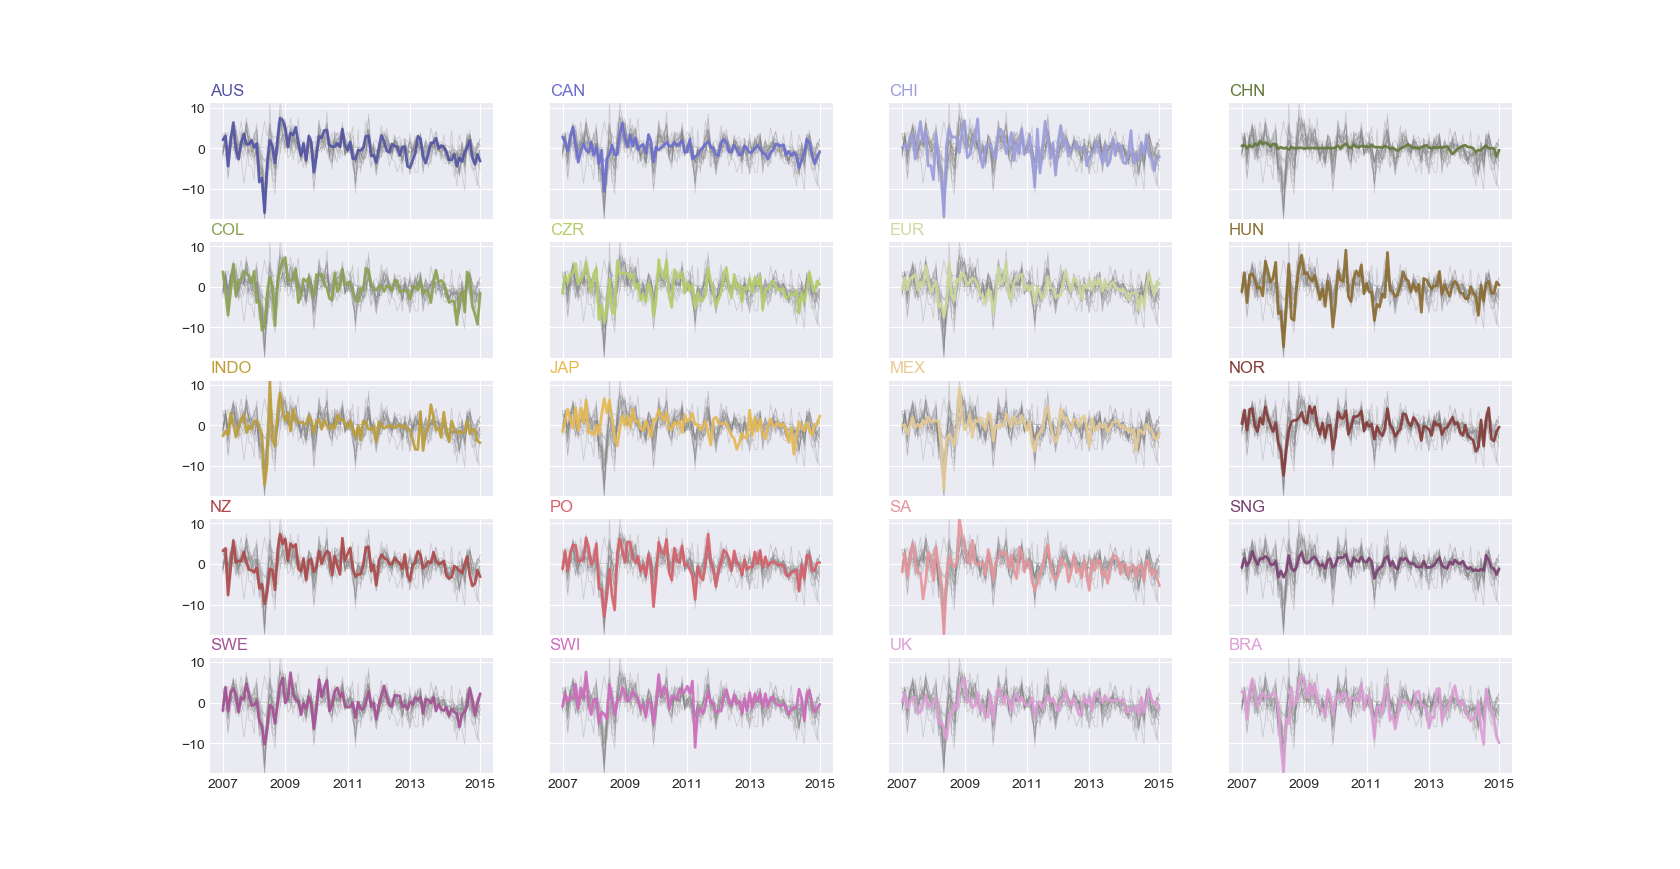
\includegraphics[scale = .8]{images/direction/er_return.png}
    \caption{Monthly Exchange Rate Return for all countries for train dataset (2007-2015)}
    \label{simulationfigure}
\end{figure}
\end{sidewaysfigure}

\newpage

In the figure above, China appears to have the least volatility in exchange rate returns. This is because China is a fixed exchange rate regime that pegs its currency against the USD. It is also interesting to see how almost all currencies faced an instant fall in excess returns during the 2008 financial crisis. This is because all currencies have USD as its base value. It seems that during the 2008 recession USD depreciated in terms of most currencies in the dataset leading to a negative return.

After calculating the exchange rate returns for each country, I used the following formula to develop a binary variable for change in foreign exchange excess returns:

\begin{equation}
  d_{t+1}^i =
    \begin{cases}
      1 & \text{if $rs_{t+1}^i  > 0$}\\
      0 & \text{if $rs_{t+1}^i <= 0$}\\
    \end{cases}
\end{equation}

In the equation above, $d_{t+1}^i$ indicate the binary variable that shows the directional change in exchange rate return at time \textbf{t+1}. Subscript \textbf{i} shows the currency being considered. The binary variable $d_{t+1}^i$ is given a value of one if the excess return is positive and it is given a value of zero if the excess return is less than or equal to zero. A value of one indicates "buy", while a value of zero indicates a "sell". This means that a trader will be recommended to buy a foreign exchange currency when the excess return is positive and sell when the exchange rate return is negative. I am going to use this binary variable to train a machine learning model that can help us make buy/sell decision based of yield curve components of a country. A buy simply shows a profit in the foreign exchange market while a sell shows loss in the foreign exchange market.

\subsection{Principal components of yield curve and its components}
Principal Component Analysis(PCA) is a dimensionality reduction machine learning technique that helps us project a multi-dimensional variable onto to a lower dimensional space. In economics, the yield curve is a curve showing several yields or interest rates for government bonds across different maturity length. A normal yield curve slopes upward, reflecting the fact that the long term interest rates are usually higher than the short term interest rate. The long term interest rate is determined by the expected future path of the short term interest rate plus a time varying bond risk premium or term premia:

\[y_{t}^n= \frac{1}{n}\sum_{i=0}^{n-1} E[y_{t+i}^1] + TP_t^n

The equation above shows a long term interest rate with \textbf{n} time period ahead maturity. The variable $E[y_{t+i}^1]$ shows the expectation of the one month interest rate \textbf{i} period ahead in the future. $TP_t^n$ shows the term premium or bond risk premium. It shows the compensation that investors require to invest in longer term bonds.

\vspace*{4mm}

The initial dataset for principal component analysis consists of the yield curve, and its expectation and term premium component. The expectation component of the yield curve informs us about the market expectation of short run yields, while the term premium component of the yield curve tells us about uncertainty and volatility in the bond market. According to the spanning hypothesis, the yield curve and its components incorporate all the valuable information about the economic situation of a country. This means that the information about all macro-economic variables of an economy are already incorporated within the yield curve \cite{salemspanning}. Hence, the yield curve and its components should have predictive power in forecasting exchange rate returns because of their ability to span different macro-economic variables related to a country. Including all maturities for yields, expectation components, and term premium components as individual variables for each country will be computationally expensive and will introduce noise into the model. The yield curve and its components sum up to 357 variables for each country. In order to reduce the dimensionality of our feature set, I am going to use PCA on yield curve and its components individually to extract their "level", "slope", and "curvature" components. According to economic literature, the first three principal components of the yield curve represent the "level", "slope", and "curvature" of all its maturities \cite{patel2018regression}. Taking the PCA of the yield curve, expectation and term premium allowed us to extract level, slope and curvature variables for each of them. The nine new variables extracted accounted for more than 95\% of the variance in our initial dataset of 357 variables. This mechanism helped us take into account all valuable information regarding all maturity levels while reducing the computation time for our models. The final nine variables that are going to be used to train our machine learning algorithms are: yield level, yield slope, yield curvature, expectation level, expectation slope, expectation curvature, term premium level, term premium slope, and term premium curvature. The following graphs shows the principal components for yield curve for all countries in the dataset:


\begin{sidewaysfigure}
  \begin{figure}[H]
      \centering
      \hspace*{-1.5in}
      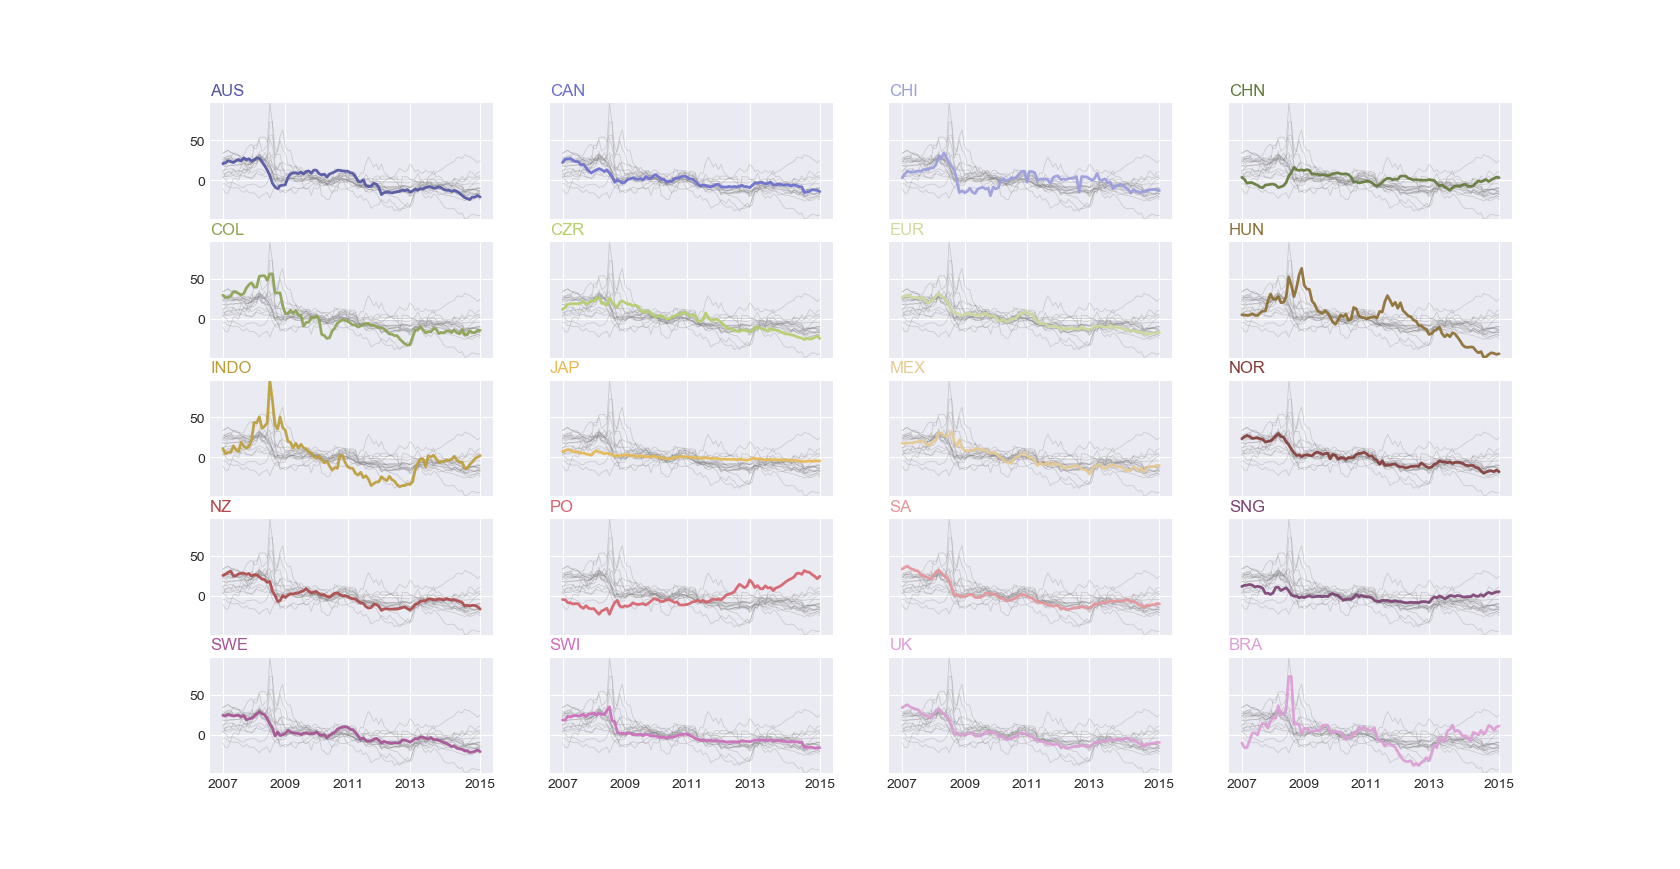
\includegraphics[scale = .8]{images/direction/yield_level.png}
      \caption{Yield Level for all countries for training dataset (2007-2015)}
      \label{simulationfigure}
  \end{figure}
\end{sidewaysfigure}


\begin{sidewaysfigure}
  \begin{figure}[H]
      \centering
      \hspace*{-1.5in}
      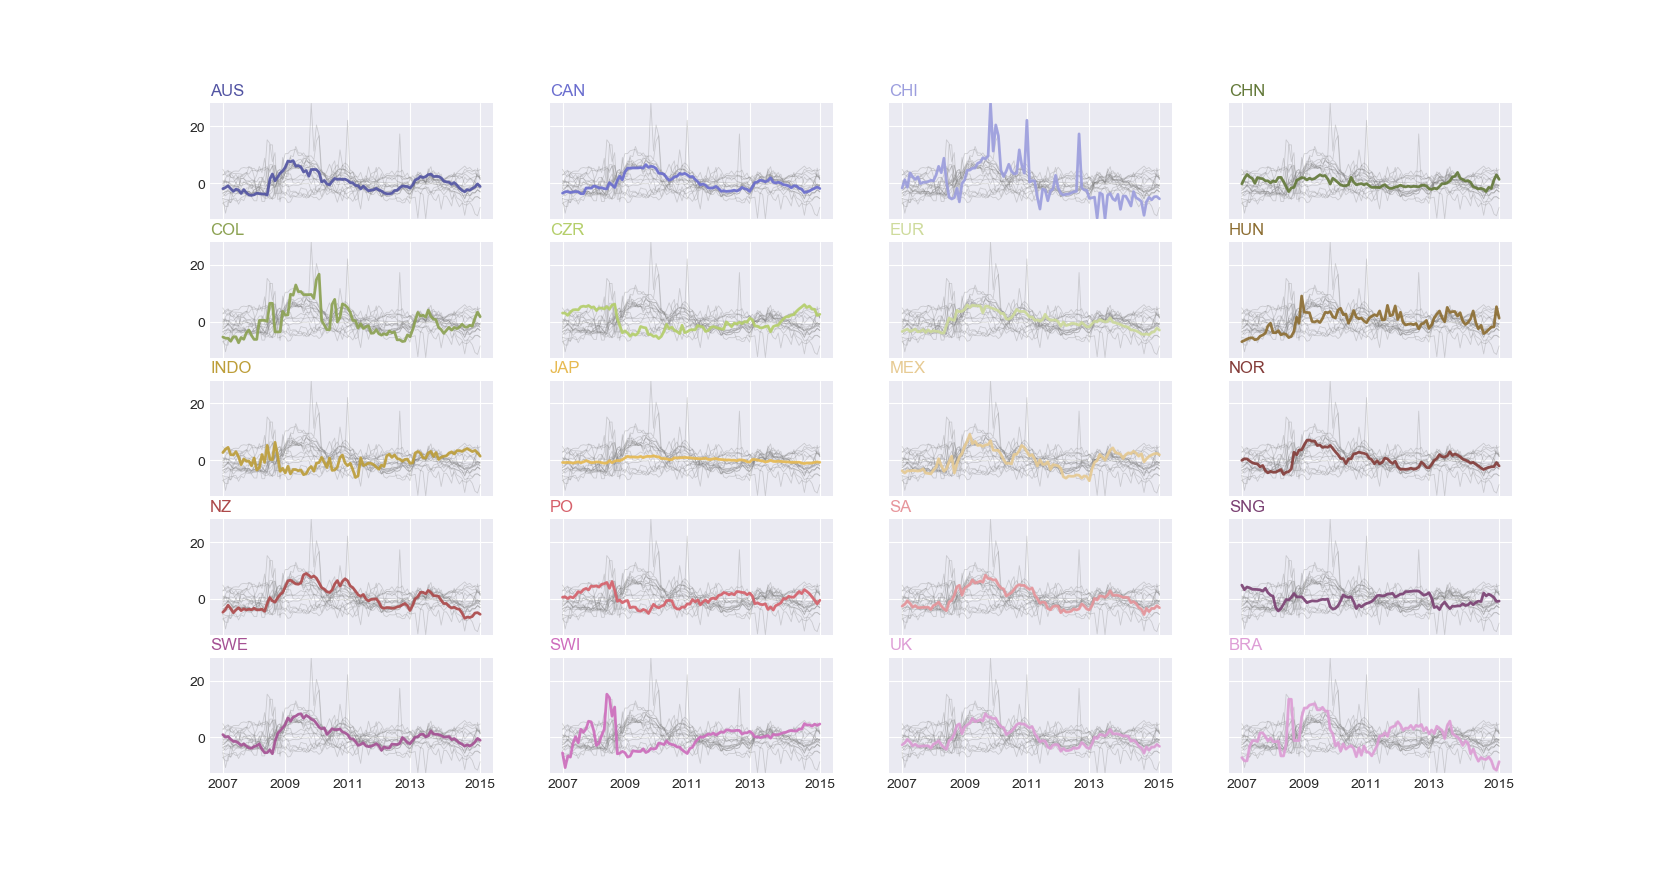
\includegraphics[scale = .8]{images/direction/yield_slope.png}
      \caption{Yield Slope for all countries for training dataset (2007-2015)}
      \label{simulationfigure}
  \end{figure}
\end{sidewaysfigure}


\begin{sidewaysfigure}
  \begin{figure}[H]
      \centering
      \hspace*{-1.5in}
      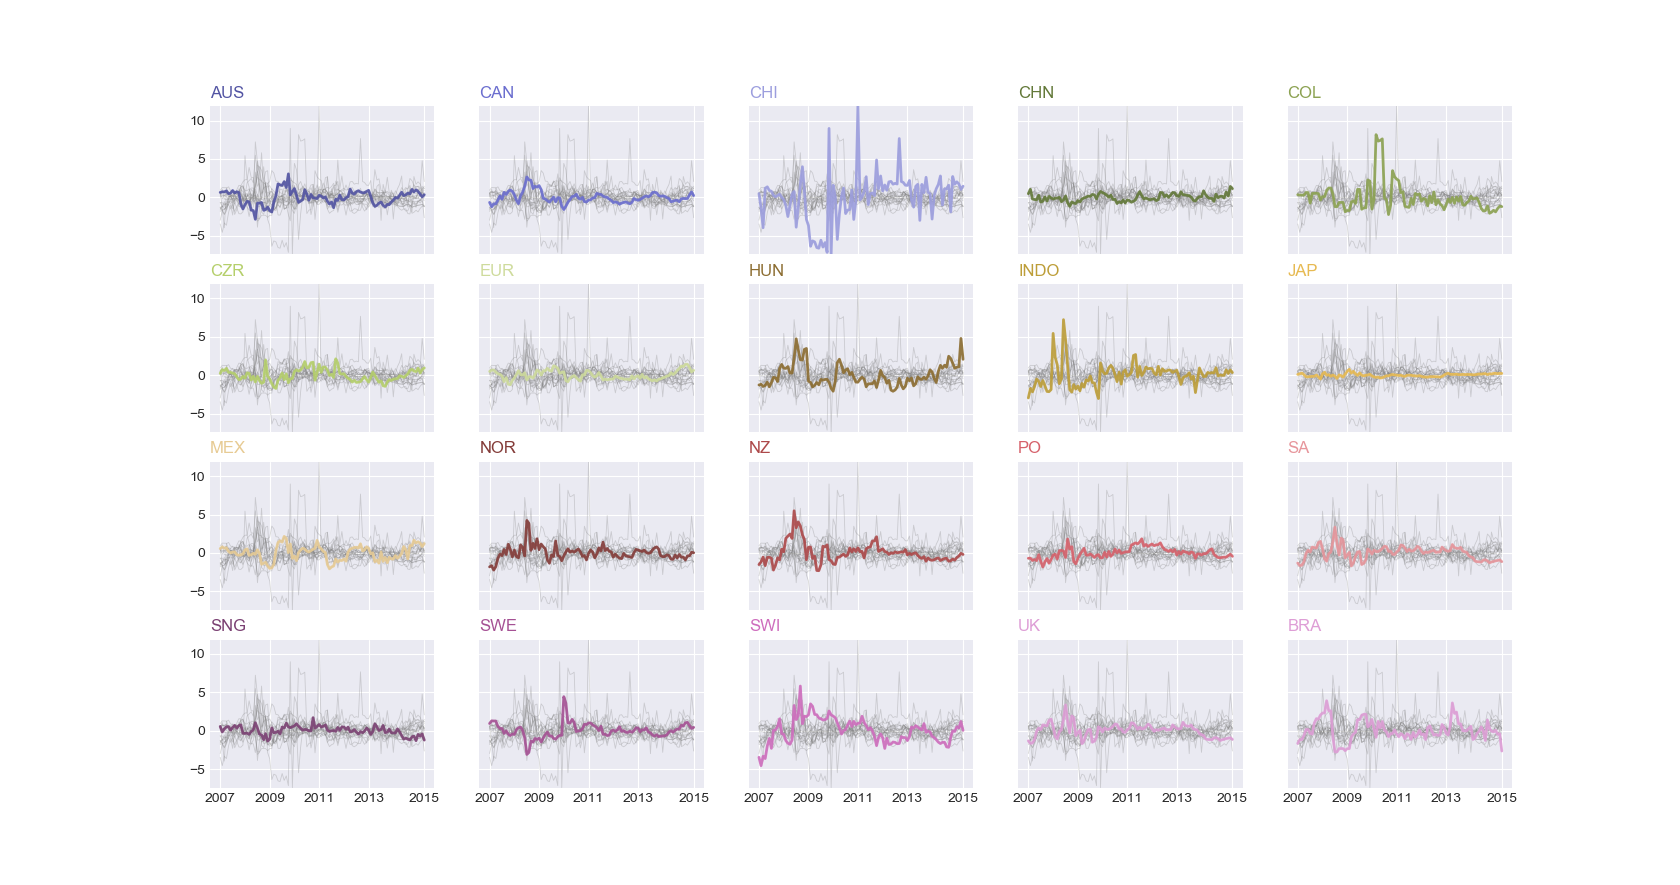
\includegraphics[scale = .8]{images/direction/yield_curvature.png}
      \caption{Yield Curvature for all countries for training dataset (2007-2015)}
      \label{simulationfigure}
  \end{figure}
\end{sidewaysfigure}

\newpage

In the figures above, China appears to be the most stable across all three principal components of the yield curve. It is also interesting to see how Chile appears relatively normal in yield level but faces drastically increased volatility in the slope and curvature component. Further economic research will be required to understand why principal components of yield curves vary across countries. This however is beyond the scope of this thesis.

\vspace*{4mm}

Similar to the yield curve, principal components for the expectation and term premium component of the yield curve were also calculated. Afterwards, the derived components for each country were differenced with that of US. This is done to calculate the economic performance of a country relative to the United States. As USD is used as the base currency for trading on the foreign exchange market. It will be valuable to look at the economic performance of a country relative to the US in order to predict the directional change in foreign exchange excess returns.

\section{Support Vector Machine (SVM)}

In this section, I am going to present the performance of the country specific SVM models developed based on our feature engineered training dataset. A support vector machine is a machine learning algorithm that is widely used for classification tasks. It is a discriminative classifier formally defined by a separating hyperplane. Given a labelled training dataset, the SVM outputs an optimal hyperplane which categorizes our dataset into buy and sell categories based on the principal components of yield, expectation, and term premium. This hyperplane is then used to categorize out of sample data by plotting it on the feature space and determining where the new data points lie compared to the hyperplane. The optimal hyperplane have \textbf{n-1} dimensions, where \textbf{n} determines the dimensions of the feature space. The hyperplane will be a line in a two dimensional vector space, a plain in a three dimensional vector space and so on. Support Vector Machines have different parameters that needs to be adjusted in order to accurately classify a dataset. A machine learning technique called Grid Search was used to identify the best parameters for our SVM model. Grid Search is the process of performing hyperparameter tuning in order to identify the best parameters for a given model. It plays an important role in machine learning as the performance of an entire model is based on the parameter values defined. After developing SVM models for predicting directional change in exchange rate return for all currencies in our dataset, I used a confusion matrix to check the performance of our models. A confusion matrix is a table that is used to describe the performance of a classification model. It creates a table that shows the true positives, false positives, false negatives, and true negatives of our model. True positive is when the model predicts a positive value when the actual value is positive. False positive is when the model predicts a positive value when the actual value is negative. False negative is when the model predicts a negative value when the actual value is positive. True negative is when the model predicts a negative value when the actual value is negative. A good performing model is one in which the number of true positive and true negatives are greater than the number of false negatives and false positives. Confusion matrices for both training and test datasets for all country SVM models were created in order to check their efficiency in predicting directional change in foreign exchange excess returns:

\begin{sidewaysfigure}
  \begin{figure}[H]
      \centering
      \vspace*{-0.75in}
      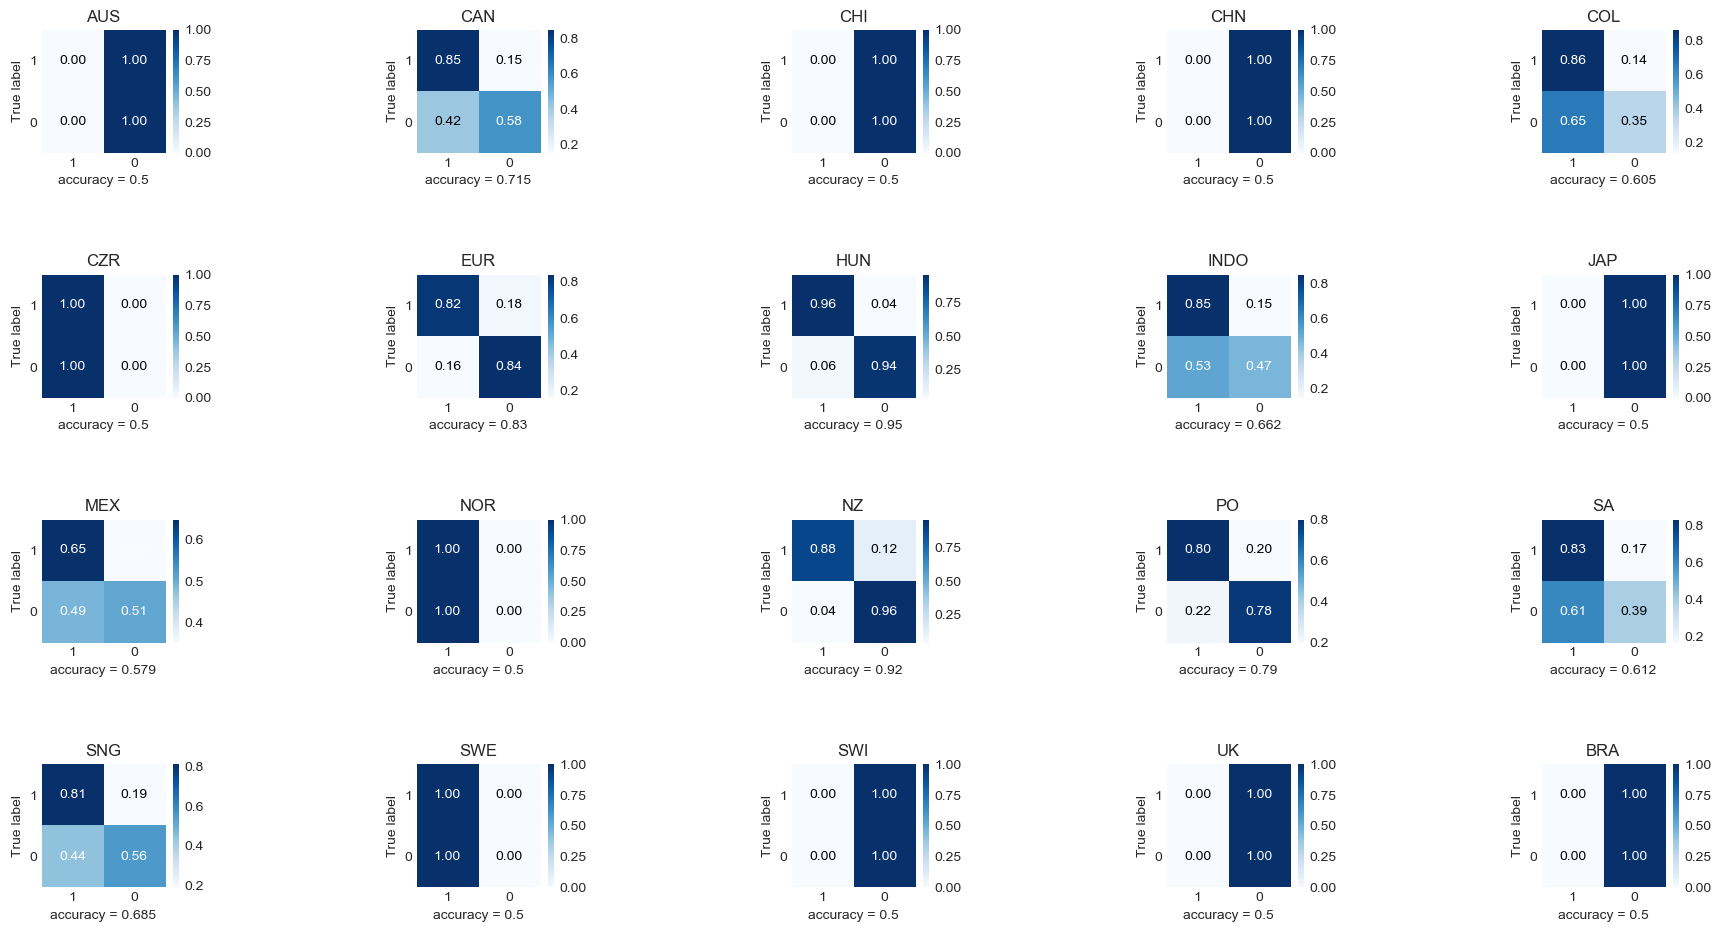
\includegraphics[scale = .45]{images/direction/clf_cm_train.png}
      \caption{SVM Confusion Matrices for all countries for Training Datasets}
      \label{simulationfigure}
  \end{figure}
\end{sidewaysfigure}

\begin{sidewaysfigure}
  \begin{figure}[H]
      \centering
      \vspace*{-0.75in}
      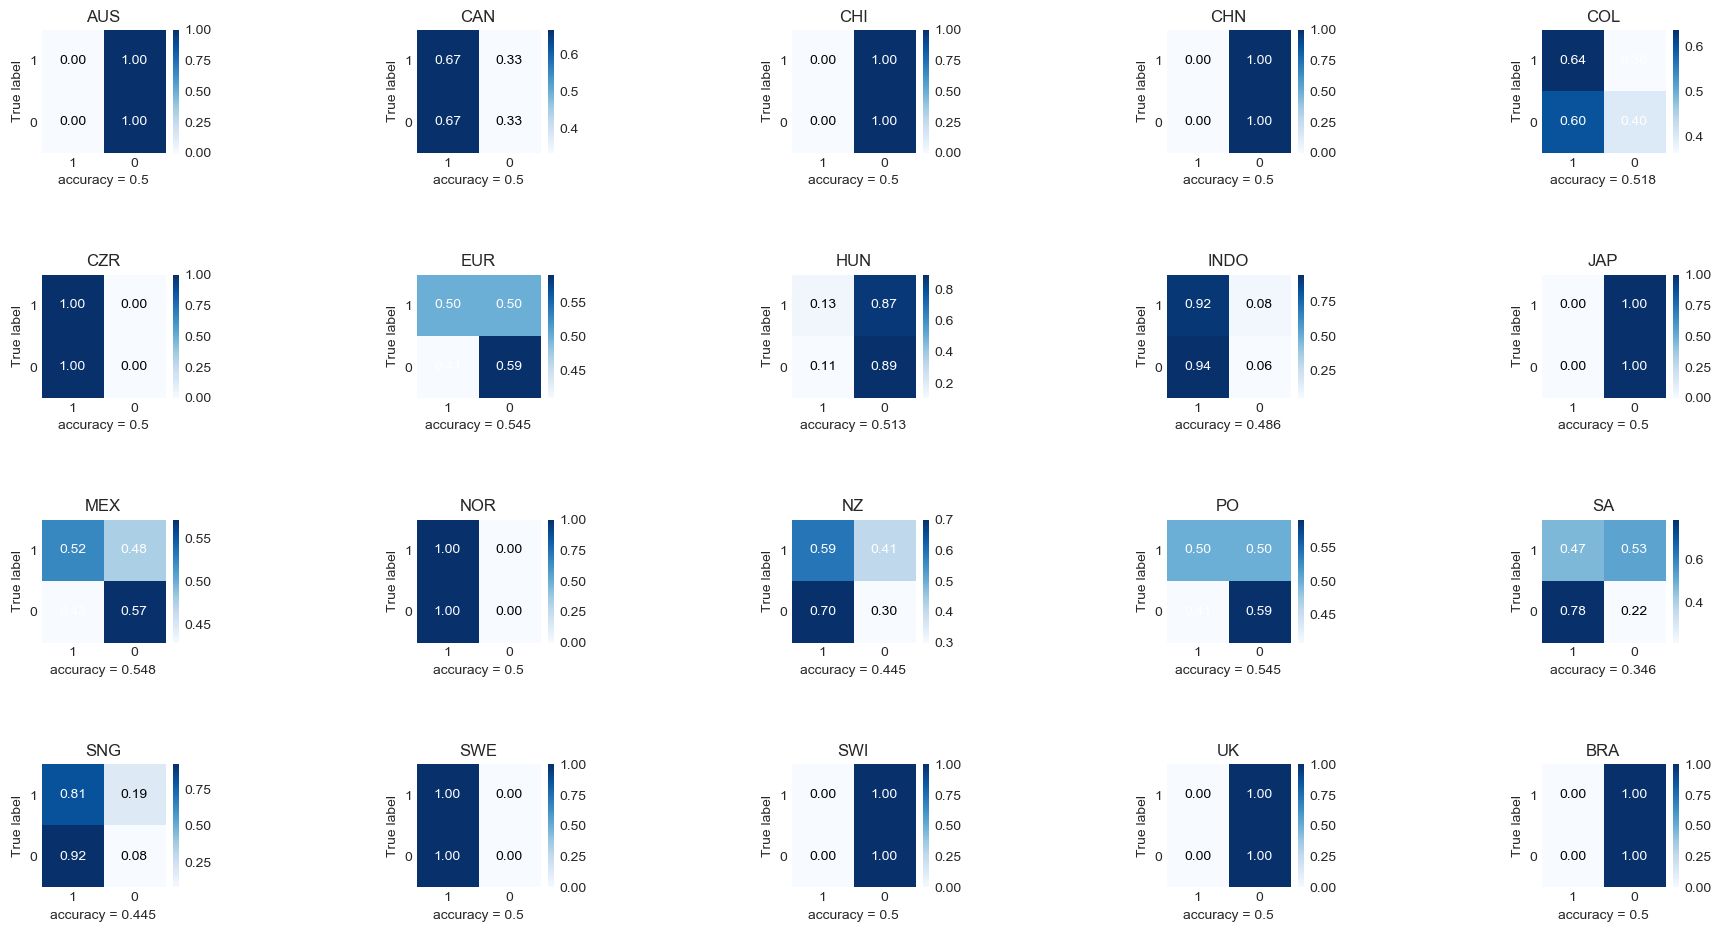
\includegraphics[scale = .45]{images/direction/clf_cm_test.png}
      \caption{SVM Confusion Matrices for all countries for Test Datasets}
      \label{simulationfigure}
  \end{figure}
\end{sidewaysfigure}

\newpage

According to the results above, most SVM models perform better than random walk on training datasets. A random walk model is equivalent to taking a random guess which, on an equally distributed dataset, will have an accuracy of 0.5 or 50\%. A model with an accuracy of 0.5 is better than a random walk model in predicting directional change in exchange rate returns. In case of test datasets, most countries act similar to a random walk model i.e. they keep predicting the same value across the time period. Only a small number of models perform better or worse than random walk in the test dataset. The difference between the performance of models on training and test datasets indicate that the models generated are not very generalizable. This means that most models do not perform well on out of sample datasets. An artificial neural network might perform better than an SVM classifier because of their ability to identify complex patterns and features in raw data.

\section{Artificial Neural Network (ANN)}
In this section, I am going to present the performance of the country specific ANN model developed based on our feature engineered training dataset. Artificial neural networks are deep learning algorithms that try to replicate how the human brain is structured. Like in a human brain, the basic building block of a neural network is a neuron that receives some input and fires an output. Similarly, an artificial neural network consists of nodes that take in values or text as input, performs some computation on them, and produces a single output value. An ANN consists of multiple hidden layers, which is a collection of nodes or neurons, with connections between different hidden layers. These layers transform data by first computing the weighted some of inputs and then normalizing the result using some kind of activation function assigned to the nodes.

\begin{figure}[H]
    \centering
    \hspace*{-0.85in}
    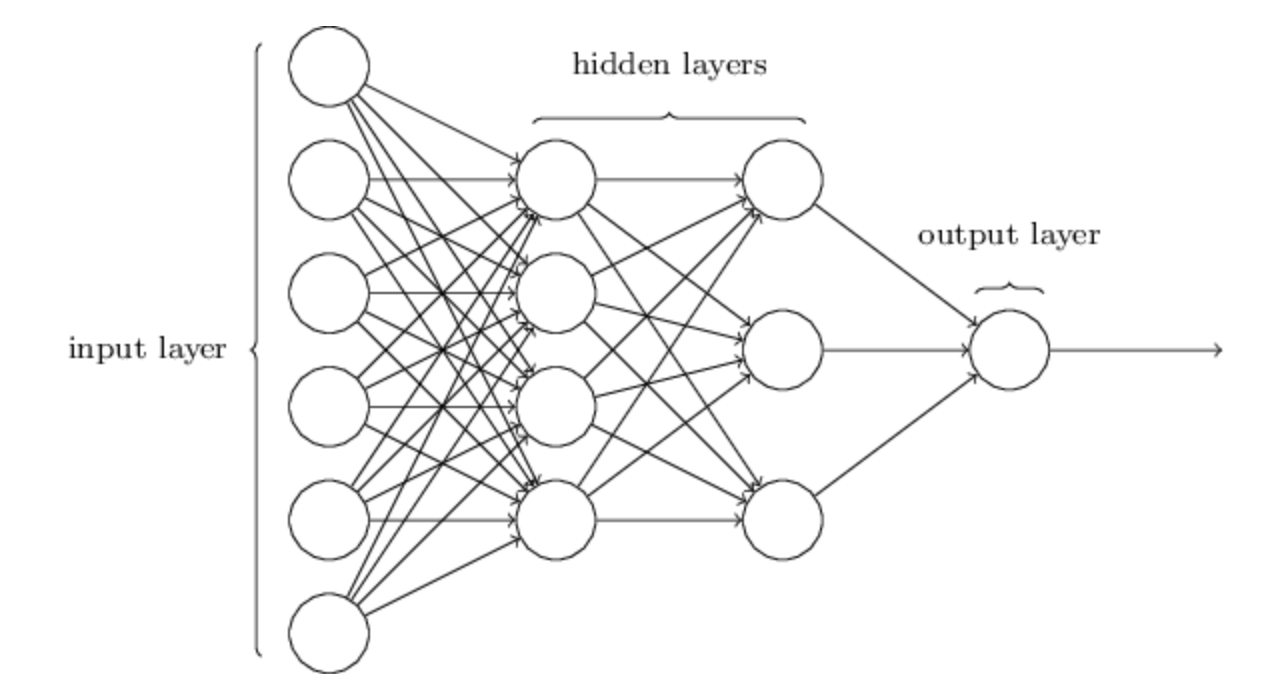
\includegraphics[scale = .45]{images/ANN.png}
    \caption{Structure of an Artificial Neural Network}
    \label{simulationfigure}
\end{figure}

A artificial neural network consists of an input layer, multiple hidden layers, and an output layer. All ANN has only one input layer and one output layer, however, the number of hidden layers between different algorithms vary based on the complexity of the problem. The input layer is where the data is entered into the algorithm, while the output layer is where the result is generated. In our case, the output layer will either generate a result of 0 or 1 based on whether the prediction is a buy or sell. Each hidden layer in the neural network can have an activation function of its own. A neural network with more than two hidden layers is called a deep neural network. A neural network makes a prediction by learning the weights of each node at every layer. The weights for each node are determined by an algorithm called \textbf{back propagation.} An ANN with two hidden layers was developed for each country in the dataset to predict the directional change in their foreign exchange returns. The first hidden layer of the neural network consists of 64 nodes, while the second hidden layer of the neural network consists of 32 nodes. A rectifier activation function is used in the hidden layers, while a sigmoid activation function is used in the output layer. Sigmoid activation function are used in the output layer for binary classification as its output values range between 0 and 1. Rectifier or ReLu activation function is the most popular activation function used for classification tasks which outputs x if x is positive and 0 otherwise. One thousand epochs were run for each model to repetitively improve the model using back propagation. Confusion matrices using both training and test datasets were created to access the performance of our ANN models in predicting directional change in exchange rate returns for a specific currency:


\begin{sidewaysfigure}
  \begin{figure}[H]
      \centering
      \vspace*{-0.75in}
      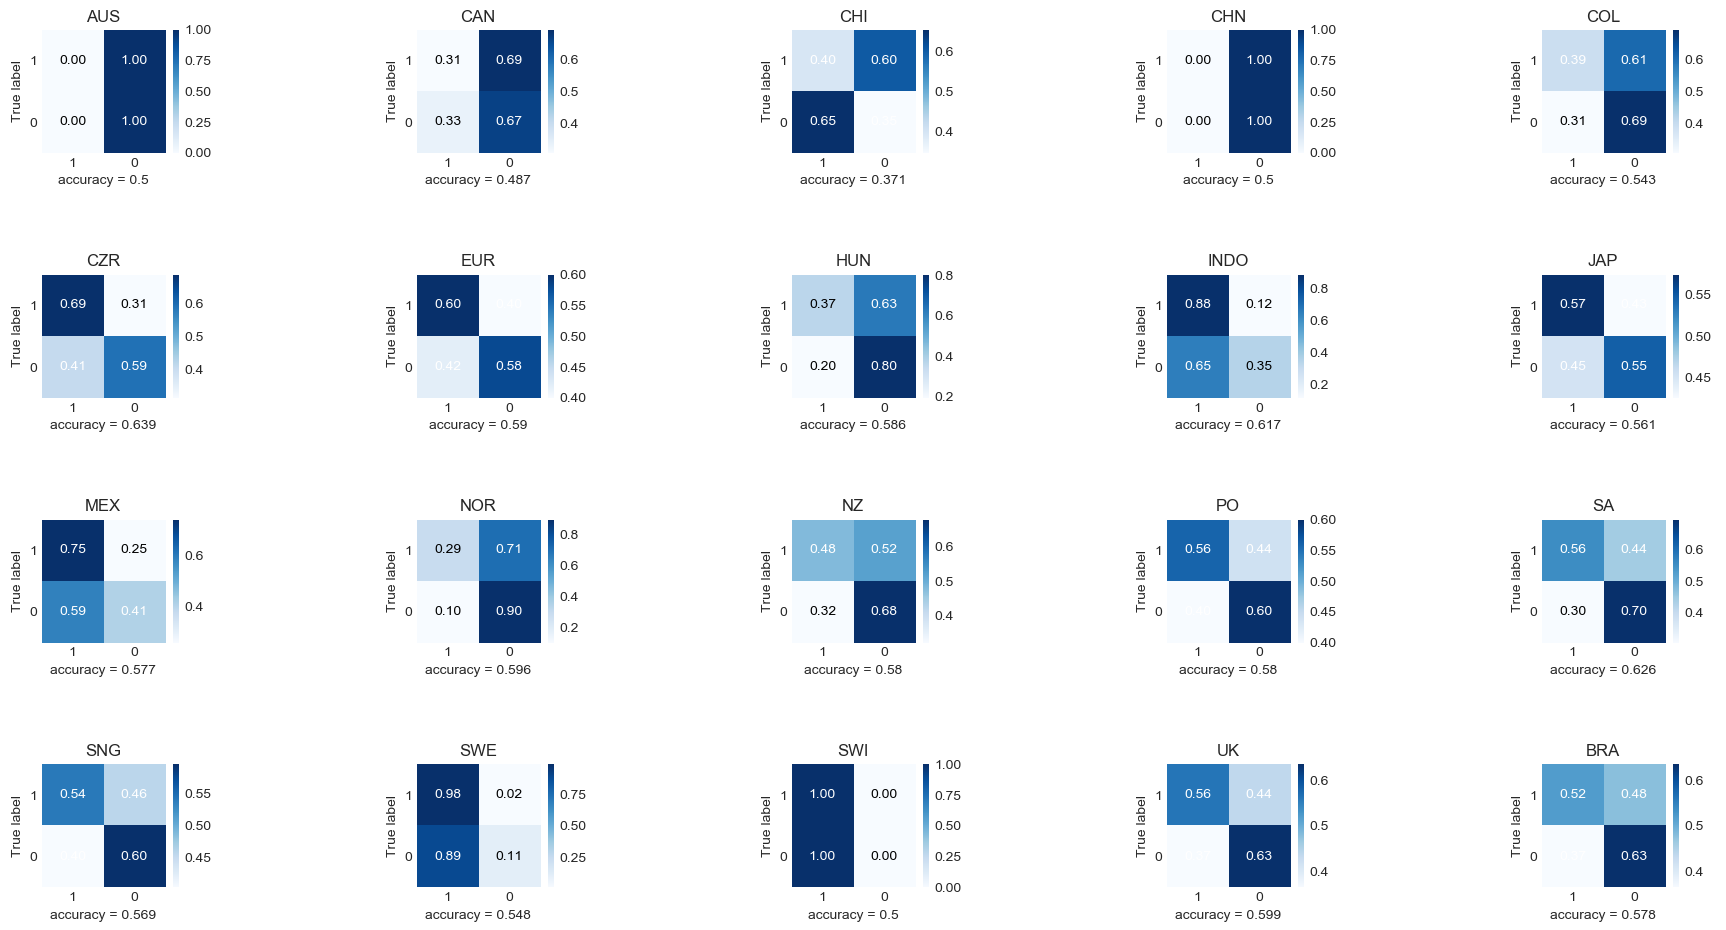
\includegraphics[scale = .45]{images/direction/n_cm_train.png}
      \caption{Neural Network Confusion Matrices for each country's Training Dataset}
      \label{simulationfigure}
  \end{figure}
\end{sidewaysfigure}

\begin{sidewaysfigure}
  \begin{figure}[H]
      \centering
      \vspace*{-0.75in}
      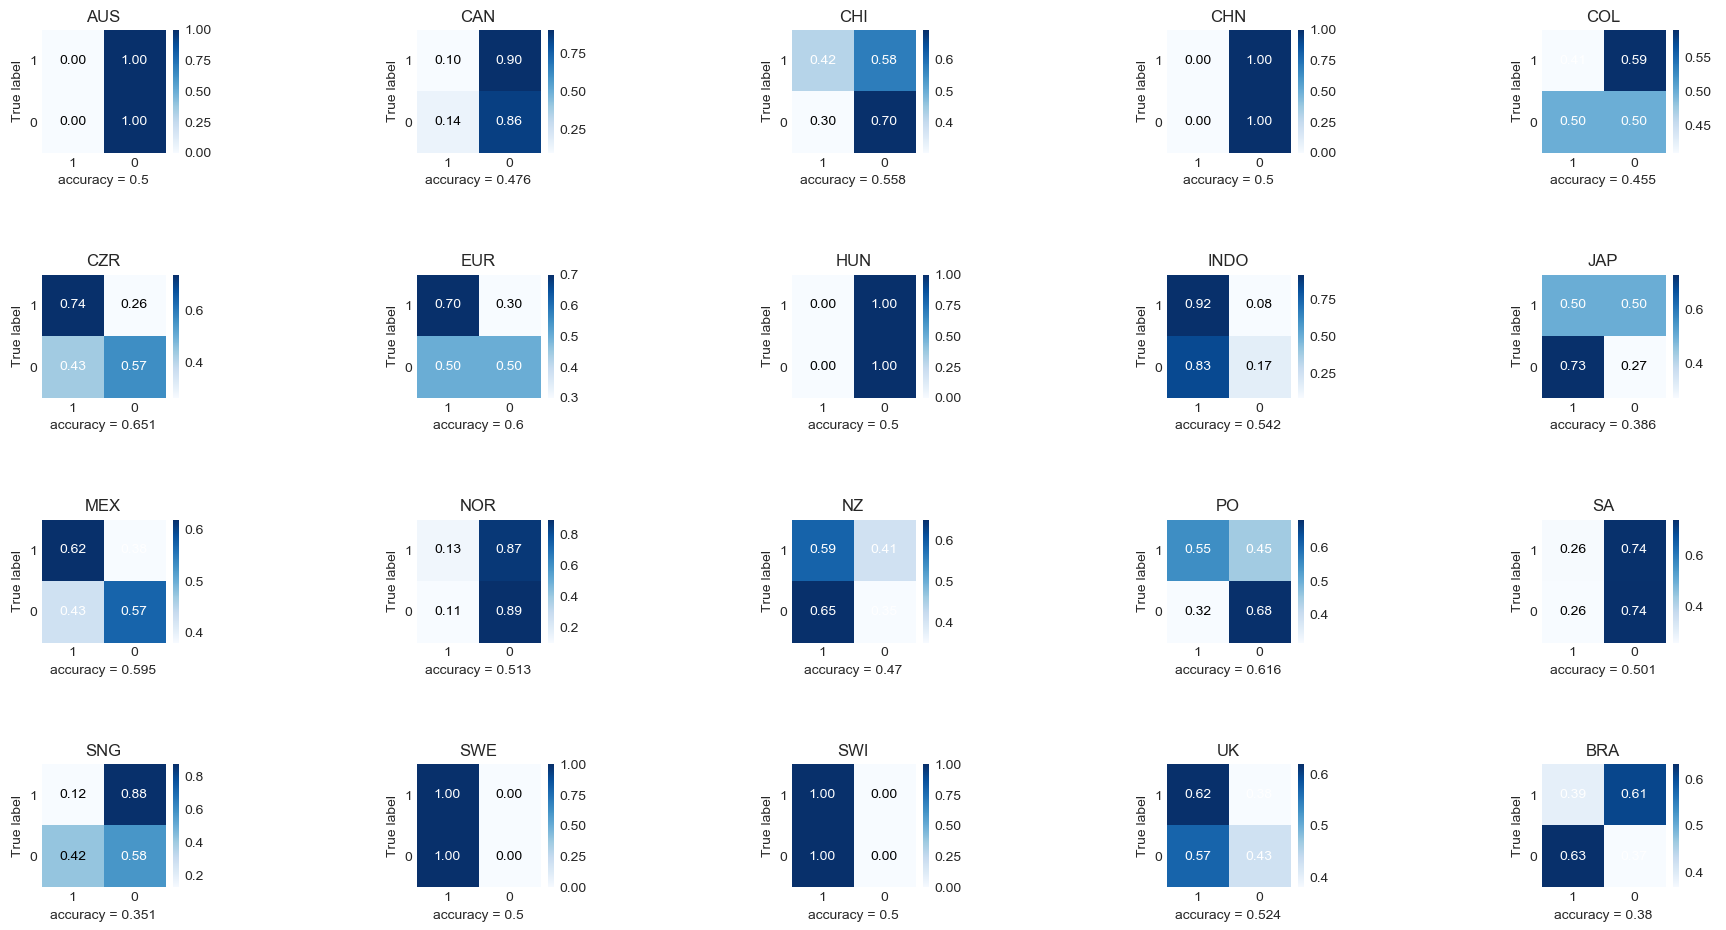
\includegraphics[scale = .45]{images/direction/n_cm_test.png}
      \caption{Neural Network Confusion Matrices for each country's for Test Dataset}
      \label{simulationfigure}
  \end{figure}
\end{sidewaysfigure}

\newpage

According to the results above, most countries' ANN models perform better than random walk on training dataset. In case of test datasets, unlike our SVM models, most countries' models perform better than the random walk. It appears that our neural network classification are more generalizable than our SVM classification models. Although our ANN model are also equivalent to random walk for many countries, this might be because of our small training dataset size. The performance of our ANN models might improve if we use hourly or daily data instead of monthly datasets.

\section{Discussion}
Artificial neural networks compared to support vector machines do a better job at predicting directional change in exchange rate returns over the short run horizon. This is because of their ability to learn abstract features from raw data. According to the financial literature, market expectations and uncertainty variables play an important role in determining directional changes in exchange rates. Hence, we might we able to improve the accuracy of our deep neural network models and SVM models by adding a sentiment variable extracted from foreign exchange news articles. Using other forms of deep learning algorithms such as convolutional neural networks or recurrent neural networks might also improve our accuracy in predicting directional change in excess returns. Convolutional neural networks are a form of deep neural networks that are mostly used to analyze visual imagery, but recently it has seen a lot of success in predicting directional change in exchange rates \cite{galeshchuk2017deep}. Recurrent Neural Networks (RNN) are deep neural networks that can use their internal state (memory) to process sequences of inputs. RNN uses the previous predicted state as an input while making new predictions which can also potentially improve the accuracy of our models. Finally, it will be useful to use hourly or daily data instead of monthly dataset as machine learning algorithms tend of perform better with larger datasets.

\chapter{Sentiment Analysis for Predicting Directional Change in Foreign Exchange Market}

Currency exchange is one of the vital components of international trade and macro-economics. The foreign exchange market is the biggest financial market in the world consisting of transactions worth billions of dollars a day (Report on global foreign exchange market activity, 2013). Traders that participate in these markets include governments, financial institutions, and retail investors."In an increasingly challenging and competitive market, having an estimate of currency movements is a holy grail" \cite{jin2013forex}. Predicting accurate directional change in the forex market is vital for formulating robust monetary policies. The predicted uptrend or downtrend of the foreign exchange market helps traders develop efficient trading and hedging strategies in the currency market \cite{galeshchuk2017}.

\vspace*{4mm}

Understanding human behavior plays a vital role in predicting directional changes in financial markets over the short run. Traders filter financial news to identify signals for trading markets. Financial markets are quite sensitive to unanticipated news articles and events. This means that we can predict directional change in currency markets by developing models to analyze financial news articles. However, identifying the effect of news articles on the currency market is an extremely challenging task. This is because of the difficulty in identifying the optimal methodology for transforming our textual data into numeric values. Econometric or machine learning algorithms can only understand data in numeric format. This makes it necessary for us to transform our textual data from text to numeric format which might cause a lose of valuable information. "Most existing literature on financial text mining or sentiment analysis relies on identifying a predefined set of keywords and machine learning techniques. These methods typically assign weights to keywords in proportion to movement of an exchange rate currency" \cite{schumaker2006textual}. Sentiment analysis is the most common natural language processing methodology used for predicting change in financial markets. Natural Language Processing is an inter-disciplinary field of linguistics, computer science, information engineering, and artificial intelligence concerned with how to program computers to process and analyze large amounts of textual data. In sentiment analysis, articles with predefined positive sentiment values (as measured by a sentiment dictionary) are related with positive change in the foreign exchange market, whereas articles with negative sentiment values are associated with negative change in the foreign exchange market \cite{calomiris2019news}. Recently, economists have started to use sentiment analysis on twitter data, google searches, and the news to predict changes in financial markets such as the stock exchange. This is because machine learning techniques are based on textual analysis tend to perform much better than linear regression or any other form of econometric models over the short run. \cite{schumaker2006textual}.

\vspace*{4mm}

Term premium and expectation components plays a vital role in predicting exchange rates over the short run horizon. Foreign exchange news articles are a great source for determining market expectation and uncertainty within the currency market. In this chapter, I am going to use sentiment analysis and natural language processing on financial news articles to predict directional change in exchange rates. Textual analysis with natural language processing is usually divided into the following steps: collecting raw data, cleaning dataset, structuring dataset, and filtering dataset. The collecting raw data stage consists of web scraping or accessing internal databases to gather textual data for analysis. The cleaning dataset stage consists of removing irrelevant textual information such as HTML tags and invalid observations. The structuring dataset stage consists of adding tags to describe our textual data (name-entity detection) and application of sentiment analysis to text. Finally, the filtering dataset stage focuses on identifying the most relevant entries that would describe a directional change in the foreign exchange market.

\vspace*{4mm}

Similar to the widely used textual analysis methodology discussed above, this chapter has been divided into the following sections: Feature Engineering, Text Preprocessing, Sorting Text by Country, Sentiment Analysis and Discussion. The feature engineering section describes all the variables used in our analysis and how they were derived. In the text preprocessing section, I am going to discuss the text cleaning techniques used to get rid of irrelevant information in our dataset. Additionally, I am also going to discuss the text to vector conversion technique used to project the textual dataset onto a vector space. In the sorting text by country section, I am going to develop an algorithm using machine learning techniques such as Word2Vec and cosine similarity to distribute financial news articles by country. In the sentiment analysis section, I am going to use five different sentiment analysis techniques to analysis the sentiment in order to predict directional change in the foreign exchange market. Finally, in the discussion section, I will end the chapter by highlighting main takeaways and discussing any further work that can be done to improve performance.

\section{Feature Engineering}
Feature engineering is the process of using domain knowledge to develop new variables and features sets that can help improve the performance of machine learning algorithms. Feature engineering is a fundamental concept in machine learning that differentiates a good model from a bad model. If done correctly, it increases the predictive power of machine learning algorithms by creating features from raw data that help facilitate the learning process. In this section, I am going to develop variables to calculate change in exchange rates and store text data based on financial news articles. The set of countries being considered are Australia, Canada, China, Chile, Czech Republic, Colombia, Hungary, Indonesia, Japan, Mexico, Norway, New Zealand, Poland, South Africa, Singapore, Sweden, Switzerland, United Kingdoms, and Brazil. The complete dataset consists of daily data ranging from 2009 to 2019. The first variable generated is the change in the exchange rate which is represented by the equation below:

\[{\Delta}s_t^i=\frac{s_t^i - s_{t-1}^i}{s_{t-1}^i}\]}

In the equation above, $\Delta s_t^i$ represents the daily change in the exchange rate for a country at time \textbf{t}. Subscript \textbf{i} indicates the currency being considered. The variable $s_t^i$ indicates the exchange rate of a country at time \textbf{t}, while the variable $s_{t-1}^i$ indicates the exchange rate of a country one period before time \textbf{t}. All foreign currencies in the dataset has USD as its base value. $\Delta s_t^i$ is the dependent variable in our model i.e. it is the variable that we are going to try to predict using sentiment analysis on financial news data.

\vspace*{4mm}

The financial news articles for our analysis were collected from investing.com using web scraping. Web scraping is technique used for extracting data from a website. The textual dataset consists of all foreign exchange news articles from 2009 to 2019 recored on daily frequency. The total dataset consists of about 82,500 news articles. The graph below shows the daily news release frequency on investing.com from 2009 to 2019:

\begin{figure}[H]
    \centering
    %\hspace*{2.5in}
    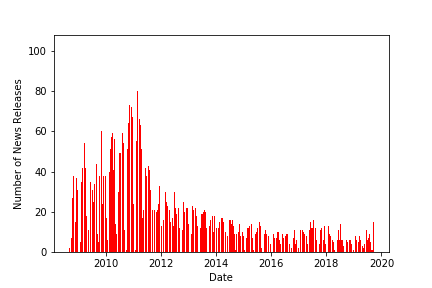
\includegraphics[scale = .99]{images/sentiment_analysis/news_frequency.png}
    \caption{Daily FOREX News Release Frequency on from 2009 to 2019}
    \label{simulationfigure}
\end{figure}

In the Figure 4.1, the daily news frequency appears to increase significantly from 2009 to 2011. This might be a result of an increase in the financial and economic uncertainty caused by the financial crisis in 2008. After around 2012, the number of foreign exchange news article release appear to go down to an average of 20 articles per day. It is expected for the number of daily news releases to increase during 2016 as a result of Brexit. This, however, does not appear to be the case. This may be a result of a drop in business for investing.com after 2012, which might be a caused by an increase in competition from financial news such as Bloomberg. In the next section, I am going to discuss the text preprocessing techniques used to prepare our news article data for sentiment analysis.

\newpage

\section{Text Preprocessing}
In order to use our news article dataset for sentiment analysis, we will need to clean it and convert it into vector format. Text cleaning allows us to eliminate any noise that might influence our analysis. Computers can only understand data in numeric format. Hence, after the text cleaning process, we will need to convert the remaining dataset into vector format using techniques such as "bag of words" or TF-IDF vectorization. This process of text cleaning and text to vector conversion is known as text preprocessing.

\subsection{Text cleaning}
Natural language processing is both a time and memory consuming process. Cleaning textual data before converting it into vectors reduces run time. It also helps us avoid extra memory allocation by getting rid of content that might introduce noise in the dataset. This helps us focus on content that is most relevant to our analysis. Text cleaning takes place in the following order:

\begin{itemize}
  \item \textbf{Removing the HTML Tags:} Our text data contains HTML tags because the dataset was scraped from investing.com (eg: $<p>$, $<h2>$ etc). HTML tags do not provide any useful insight during the sentiment analysis process. It is important to get rid of them in order to eliminate noise into the dataset.

  \item \textbf{Removing Punctuations:} Similar to HTML tags, punctuation adds unnecessary extra detail. Hence it is a good idea to eliminate them in order to save memory space and computational time.

  \item \textbf{Removing Stop words:} Stop words like "this", "there", "is", "make" etc can also be unnecessary. However, it is important to be cautious while getting rid of stop words like "not" because they can be critical to interpreting data.

  \item \textbf{Stemming:} This is the process of extracting root words from a text. Words like "tasteful", "tastefully" etc are all variations of the word "tasty". Instead of having to create a vector for each of these words, it is better to stem all the words to their root as it helps better analyze and interpret the textual dataset.

  \item \textbf{Lemmatization:} Similar to stemming, lemmatization is used to convert a word back to its base form. However, this process uses a dictionary for vocabulary and morphological analysis of words. While stemming processes words individually, lemmatization also considers the context in which it is being used. Lemmatization, for example, can identify that "good" is the base form of 'better' while stemming will not account for this.

  \item \textbf{Converting words to lower case:} Words like "Biscuit" and "biscuit" are classified differently because computers cannot differentiate between the uppercase and lowercase form. For this reason, it is important to convert all textual data to lower case form in order to enhance model performance.

\end{itemize}


\subsection{Text to vector conversion}
Next, we will need to convert the dataset into numeric or vector form. There are multiple techniques that can be used to project text onto a vector space. The three techniques used in this paper are:

\begin{itemize}

  \item \textbf{Bags of Words:} This is the simplest method for projecting text onto a vector space. This technique creates a dictionary of "n" words where "n" is the number of unique words in our text corpus. It then creates an "n" dimensional vector for each of our documents in the dataset. Each cell (or dimension) in the bag of words has a value representing the number of times the corresponding word has occurred in the document. As the vocabulary of the whole dataset increases, the number of dimensions in the bag of words also increases. This means that for each document in a big dataset the number of zeros will exceed the number of non-zeros. Vectors which contain a majority of zeros are referred to as sparse vectors. Many sparse vectors stacked on top of each other create a grouping called a sparse matrix.

  \item \textbf{Term Frequency-Inverse Document Frequency (TF-IDF):} This is a more advanced text to vector conversion technique that contains two concepts: Term Frequency (TF) and Inverse Document Frequency (IDF). Term Frequency (TF) refers to the frequency of a word appearing in a document. TF aims to identify words that occur the most in a document. It can be represented as:

\[TF=\frac{Number \: of \: times \: a \: word \: appear \: in \: the \: document}{Total \: number \: of \: words \: in \: the \: document}\]}

Inverse Document Frequency(IDF), on the other hand, aims to find the importance of a word by checking its uniqueness across the complete dataset. IDF is based on the idea that words that are less frequent across the documents but frequent within a specific document are critical to understanding that specific document.

\[IDF=log_{10}\frac{Total \: number \: of \: documents}{Number \: of \: documents \: in \: which \: word \: appears}\]}

TF-IDF is a multiplication of the TF and IDF equations. It aims to identify the words that are unique to a specific document in order to better understand the content of a text. Multiplication of TF with IDF helps reduce the values for high frequency common words that occur across most of the dataset. It is a powerful technique that can be used for classifying text with different writing styles because it can identify words that are unique to a document.

  \item \textbf{Word2Vec:} This is the most advanced and time consuming text to vector conversion technique among Bags of Words and TF-IDF. Word2Vec consists of all the deep learning models that can be used for generating word embedding. A word embedding is an approach for providing a dense vector representation to a set of words that captures something about their meaning. The vector space representation of the words provide a projection where words with similar meanings are clustered together. These models consist of a shallow two layer neural network with one input layer, one hidden layer and one output layer. It is through the use of these pre-trained neural networks that we can generate word embeddings for textual data. The two main architectures utilized by Word2Vec models are Continuous Bag of Words (CBOW) and Skip Gram. It is through the use of these word embedding techniques over other word to vector conversion techniques that has lead to breakthrough performance with deep neural networks on problems such as machine translation.

\end{itemize}

\newpage

\section{Sorting Text by Country}

After preprocessing foreign exchange news articles, I am going to sort them by country in order to perform currency specific sentiment analysis. The list of countries that are being considered are Australia, Canada, Chile, China, Colombia, Czech Republic, Hungary, Indonesia, Japan, Mexico, Norway, New Zealand, Poland, South Africa, Singapore, Sweden, Switzerland, United Kingdoms and Brazil. The complete textual dataset contains about 82,500 news articles. It would be very time consuming (and almost impossible) to manually go through all the articles and group them by country. For this reason, I developed a sorting mechanism that searches for country specific words in a document along with word embedding and cosine similarity to incorporate any document that might have been left out. A combination of straight forward searching and cosine similarity based searching is used to optimize sorting efficiency. Both the techniques are explained below:

\begin{itemize}

  \item \textbf{Search for specific country related terms:} This method involves searching through all the documents in the dataset for country specific search terms. To do this, I first developed a specific list of search terms for each country with the following format: $[country\: name, currency\: code, citizenship]$. Every country had these three words in their list of search terms. For example, in case of Australia the search terms were $[australia, aud, australian]$. After creating a list of search terms, every document in the dataset was looped over in order to identify country specific news articles. Every document was classified into a different country based on the search terms it contained. Finally, all the results were organized into separate news article data frames for each country.

  \item \textbf{Search based on cosine similarity:} Simply searching for specific search terms to classify data is not the most effective way to sort textual data by country because their always remains a possibility that we might be missing some country specific search terms that are important for grouping our news articles. This means that there is always a chance of leaving out articles that are related to a country. In order to minimize the probability of misclassifying valuable news articles, I combine the searching process with a text similarity technique called cosine similarity. Text similarity is the process of determining how "close" two pieces of text are, both in lexical (surface closeness) and semantic (meaning) similarity. These techniques make use of word embedding to represent documents in multi-dimensional vector space and compare documents by measuring the distance between the vectors in the feature space. Cosine similarity is one of the most widely used methods for text similarity. It calculates the similarity between texts by measuring the cosine of the angle between two vectors. The cosine similarity index ranges from 0 to 1 where 0 indicates the least similar, while 1 indicates perfect similarity. It is beneficial to use this technique while sorting data by country because it enables us to account for any country specific terms that might have been missed. For example words like "Toronto" and "Ontario" have more than 0.5 cosine similarity with "Canada". This means we can simply use a country name along with cosine similarity to search for all articles relating to it. In order to apply the technique based on cosine similarity, each document in the dataset was projected on a vector space using Word2Vec. Afterwards, the same country specific search terms used in previous searching methods were also projected onto a vector space. Finally, any document containing text that had a cosine similarity of more than 0.5 with a specific country's search term was classified accordingly. All results were organized into country specific dataframes.

  \item \textbf{Combining both search results:} Once individual news article dataframes for each country were created, using both simple and cosine similarity searching methodologies, the resulting data frames were merged together. In the case where each of the two strategies classified the same document to one country, the resultant dataset contained duplicate content. In order to prevent any duplication in the final dataset for each country, observations that occurred more than once in the dataset were eliminated.

\end{itemize}

\subsection{Textual Data Structure}

The following table shows the length of country specific news article datasets that were created after combining the results of simple and cosine similarity searching methodologies:

\vspace*{6mm}

\begin{center}
\begin{tabular}{ |p{3cm}||p{3cm}|p{3cm}|p{3cm}|  }
 \hline
 \multicolumn{2}{|c|}{Dataset Lengths} \\
 \hline
 Country Code & Number of articles \\
 \hline
 AUS   & 26074\\
 CAN   & 30591\\
 CHI   & 331\\
 CHN   & 15634\\
 COL   & 3978\\
 CZR   & 1297\\
 EUR   & 64807\\
 HUN   & 1183\\
 INDO  & 1024\\
 JAP   & 38023\\
 MEX   & 2365\\
 NOR   & 641\\
 NZ    & 14524\\
 PO    & 929\\
 SA    & 5515\\
 SNG   & 8618\\
 SWE   & 1211\\
 SWI   & 17158\\
 UK    & 34530\\
 BRA   & 1791\\
 \hline
\end{tabular}
\end{center}

\vspace*{8mm}

According to the table above, the Euro based countries appears to have the largest number of articles, followed by Japan and United Kingdom. Chile, on the other hand, appears to have the least amount of FOREX news articles, followed by Norway and Poland. This shows that most of the articles in our dataset focus on the exchange rate of European countries, Canada, Japan and China.

\vspace*{4mm}

Machine learning and deep learning techniques for text analysis perform better on bigger datasets. The performance of a machine learning model is directly proportional to the size of its training dataset. This is because large datasets consist of more observations that can be used to train a model. In order to make sure that our sentiment model for each country has enough training datasets, I decide to get rid of any country that has less than 3000 articles. This left us with the following eleven countries:

\vspace*{6mm}

\begin{center}
\begin{tabular}{ |p{3cm}||p{3cm}|p{3cm}|p{3cm}|  }
 \hline
 \multicolumn{2}{|c|}{Dataset Lengths} \\
 \hline
 Country Code & Number of articles \\
 \hline
 AUS   & 26074\\
 CAN   & 30591\\
 CHN   & 15634\\
 COL   & 3978\\
 EUR   & 64807\\
 JAP   & 38023\\
 NZ    & 14524\\
 SA    & 5515\\
 SNG   & 8618\\
 SWI   & 17158\\
 UK    & 34530\\
 \hline
\end{tabular}
\end{center}

\subsection{Effectiveness of text sorting algorithm}

In order to check for the effectiveness of the news article distribution among countries, I make use of word clouds to visualize the highest frequency words in each country's dataset. Ideally, every country's word cloud should have words relating to its economic and financial components. The extent to which we can distinguish between the word clouds of each country determines the effectiveness of our sorting mechanism. More distinguishable word clouds indicate effective performance of our sorting algorithm.

\begin{figure}[H]
    \centering
    %\hspace*{2.5in}
    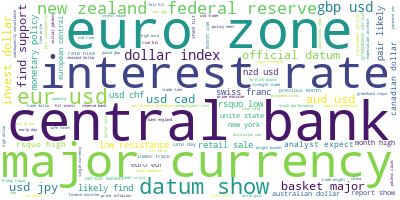
\includegraphics[scale = .95]{images/sentiment_analysis/CAN_wordCloud.png}
    \caption{Word Cloud of top 100 words for Canada}
    \label{simulationfigure}
\end{figure}

\begin{figure}[H]
    \centering
    %\hspace*{2.5in}
    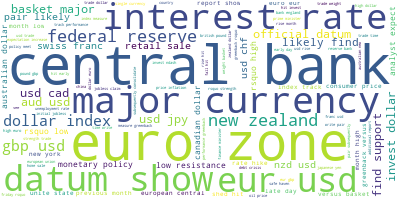
\includegraphics[scale = .95]{images/sentiment_analysis/CHN_wordCloud.png}
    \caption{Word Cloud of top 100 words for China}
    \label{simulationfigure}
\end{figure}

\begin{figure}[H]
    \centering
    %\hspace*{2.5in}
    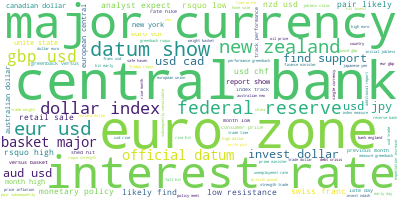
\includegraphics[scale = .95]{images/sentiment_analysis/JAP_wordCloud.png}
    \caption{Word Cloud of top 100 words for Japan}
    \label{simulationfigure}
\end{figure}

The figures above show word clouds for Canada, China, and Japan respectively. Our sorting mechanism is efficient if word cloud for each country can easily be distinguished. This, however, does not appear to be the case. The word clouds for China, Canada and Japan do not appear to vary greatly. This indicates that our sorting mechanism was not very efficient. It is understandable that "interest rate" is the most frequent term but words like "Euro Zone" which are not directly related to China and Japan's currency should not occur in their respective word clouds. Every country's word cloud not only appears to have a mention of its own currency but also that of other currencies. This leads to the introduction of noise in our textual datasets which can cause our sentiment model to misclassify one country's sentiment with that of another. The word clouds above show that our strategy for sorting text by country was not very effective. This can influence our sentiment analysis results as our datasets might not be representative of the countries being considered. It will be vital to reconsider our text sorting mechanism if the exchange rate directional forecasting results with textual data are not significant.

\section{Sentiment Analysis}
Sentiment Analysis is a subfield of Natural Language Processing that aims to determine whether a piece of text is negative, positive or neutral in tone. This is also known as opinion mining or emotion AI. Sentiment Analysis helps us convert unstructured text data into structured data that can then be used to train a model. Sentiment analysis is widely used in asset pricing and financial market analysis because of the importance of expectation component in predicting different financial variables such as exchange rates and stock prices. News articles and social media are known to be one of the major drivers of expectation in the financial markets. Machine learning algorithms cannot directly understand a news or social media article. They require sentiment analysis or some other similar natural language processing technique to covert data into a processable format. Sentiment analysis informs us about the polarity of a news paper article which can then be used to determine the directional change in exchange rate or any other asset prices. Sentiment Analysis can be applied at different scope levels:

\begin{itemize}
  \item \textbf{Document Level:} sentiment analysis used to obtain the tonality of a complete document, article or paragraph.
  \item \textbf{Sentence Level:} sentiment analysis used to obtain the tonality of a single sentence.
  \item \textbf{Sub-sentence Level:} sentiment analysis used to obtain the tonality of sub expressions within a single sentence.
\end{itemize}

In my analysis, I am going to use document level sentiment analysis as the text dataset consists of daily foreign exchange news articles. In order to bring everything to daily frequency for predicting directional change, I combined all articles issued on the same day into a single document. This makes sure that we have one document for each day and the sentiment analysis for that document would represent the overall tonality of that particular trading day. This overall sentiment can then be used to predict future daily directional change in exchange rates.

\subsection{Methods for Sentiment Analysis}

There are many methods and algorithms that can be used to implement sentiment analysis systems on textual data. They can be classified as follows:

\begin{itemize}
  \item \textbf{Rule based} systems perform sentiment analysis based on a set of manually determined rules. A basic rule based system usually works from the face of a predetermined dictionary of positive and negative words. The dictionary is used to identify the number of positive and negative words occurring in a document. If the number of positive words are greater than the number of negative words then the document is classified as positive or else it is given a negative sentiment. A neutral sentiment score is given when the number of negative and positive words in a document are the same. This is the basic form of rule based sentiment analysis. Other advanced rule based sentiment analysis use different techniques such as assigning different weights to specific positive and negative words i.e. words that are extremely negative or positive are given more weight in a document than those that are more neutral. This helps make our model more dynamic as all negative and positive words in our dictionary are not treated the same.

  \item \textbf{Automatic} systems rely on machine learning and deep learning techniques to learn from textual data. Unlike Rule based systems, they do not depend on manually crafted rules for sentiment analysis. In the case of automatic systems, the sentiment analysis task is usually modeled as a classification task. This means that for automatic systems it is important to use an already pre-labeled training text dataset. The training dataset is used to fit a machine learning classification model such as Support Vector Machines, Neural Networks, or Logistic Regression. These trained models are then used to predict the tonality of new unstructured text data that does not have any labels. The image below shows how the training and prediction process of automatic systems for sentiment analysis work:

  \begin{figure}[H]
      \centering
      %\hspace*{2.5in}
      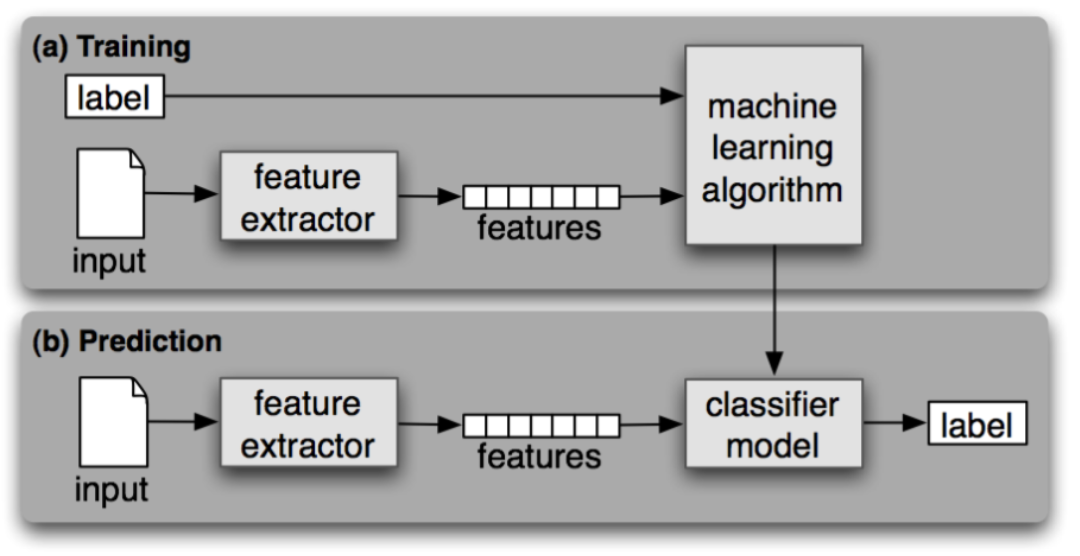
\includegraphics[scale = .42]{images/sentiment_analysis/automatic_systems.png}
      \caption{Training and Prediction Process of Automatic Systems for Sentiment Analysis}
      \label{simulationfigure}
  \end{figure}

During the training process of automatic systems, the textual data is considered as input while the sentiment labels (positive, negative, and neutral) are considered as labels. The labels and text data is split into a training and test set in order to check for overfitting after the model has been created. The text data is passed through the feature extractor before being fed into the machine learning algorithm. The feature extractor executes the text preprocessing tasks by cleaning the textual dataset and using text to vector conversion. Once the training dataset is in vector format, it is fed into the machine learning classification algorithm along with its respective labels. After training the model, we use the test dataset to check for the out of sample performance of our machine learning algorithm. Checking our model with a test dataset helps us make sure that our model is generalizable and not overfitting to the training dataset. After a suitable model has been developed, we can use it to predict the labels of new unstructured textual data. Now we can use our model to predict the tonality of any new text documents. Deep learning automatic systems work best for sentiment analysis if provided with huge training and test datasets. Most people do not train their own automatic systems for sentiment analysis as it is very time consuming and computational expensive to train a deep learning sentiment analysis model. Instead most of the automatic systems used today are pre-trained by large data science and Artificial Intelligence corporations.

  \item \textbf{Hybrid} systems combine both the rule based and automatic approaches. Hybrid systems can gain higher precession and accuracy by combining the best of both worlds.

\end{itemize}

\subsection{Models for Sentiment Analysis}

In this section, I am going to discuss the models that I used for sentiment analysis on the news articles dataset. A combination of rule based and automatic sentiment analysis systems are used in an effort to identify the best sentiment extraction technique for predicting short run directional change in exchange rates. Following is the list of sentiment analysis techniques that were used:

\begin{itemize}
  \item \textbf{Tonality Dictionary} is a rule based system with 231 positive words and 102 negative words in its dictionary. The sentiment analysis dictionary for this model is adapted from the paper 'What's the Story? A New Perspective on the Value of Economic Forecasts' where the authors use it to measure the degree of optimism and pessimism regarding Federal Reserve Board forecasts published in the Greenbook \cite{sharpe2017s}. The model uses a tf-idf weighting scheme along with the dictionary of positive and negative words for conducting sentiment analysis on foreign exchange news articles. A sentiment score that is greater than 0 is considered to be positive while anything less than 0 is considered negative. A score of exactly 0 is considered to be neutral (which is rarely the case.)

  \item \textbf{VADER} stands for Valence Aware Dictionary and sEntiment Reasoning. It is an open source pre-trained algorithm that works off a simple rule based model for conducting sentiment analysis. It was created and optimized for sentiments expressed on social media like twitter, online news, movie/product reviews etc. Furthermore, VADER is also able to include sentiments for emoticons (e.g. :D), acronyms (e.g. LoL) and slang. I decided to use VADER for sentiment analysis on FOREX news articles because of its reputation for performing well on online media including news articles. The compound score in VADER's result is an aggregate of negative, positive and neutral sentiment scores of a text. If the compound score of a document is greater than or equal to 0.05, it is considered to be positive. On the other hand, if the compound score of a document is less than or equal to -0.05, it is considered to be negative. Anything between -0.05 to 0.05 is considered neutral.

  \item \textbf{TextBlob} is a python package that can be used for sentiment analysis. It is a rule based system that works well with negation and modifier words. This means that it is able to classify "great" as positive while "not great" as negative. It also understands modifiers which means that it will assign a higher positive sentiment score to "very great" than "great". It ignores one letter words in its sentiment phrases which means that sentences like "not a very great" will be assigned the same negative sentiment score as "not very great." Lastly, it also ignores any words that does not exist its dictionary. This means that it will assign the same negative sentiment score to "not a very great calculation" as it will to "not a very great". I decided to use it as one of my models for sentiment analysis because of its capacity to understand different text structures that play a role in tonality extraction. A sentiment score that is greater than 0 is considered to be positive while anything less than 0 is considered negative. A score of exactly 0 is considered to be neutral (which is rarely the case.)

  \item \textbf{Harvard IV-4 Dictionary} is a tonality dictionary developed by Harvard University that is most widely used for sentiment analysis as it contains a vast list of positive and negative words. I used the dictionary to develop a rule based system that assigns a score of greater than 0 for positive sentiment, a score of less than 0 for negative sentiment, and a score of 0 for neutral sentiment.

  \item \textbf{Loughran and Mcdonald (LM) Dictionary} is a dictionary developed specifically for the accounting and financial domain. According to Loughran and McDonald (2011), applying a general sentiment word list to accounting and financial documents can lead to high rate of misclassification \cite{loughran2011liability}. It is for this reason that they developed a custom financial dictionary of positive and negative words. They also added an uncertainity word list that attempts to measure the general notion of imprecision. The financial dictionary contains 2339 negative words and 353 positive words. I used the LM dictionary to develop a rule based system that assigns a score of greater thatn 0 for positive sentiment, a score of less than 0 for negative sentiment, and a score of 0 for neutral sentiment.

  \item \textbf{Aggregate Sentiment} system determines the sentiment of an article by averaging the sentiment score of all five models discussed above. The aggregate sentiment systems is an ensemble method that aims to tap into the strengths of all previous models. Ensemble models are meta-algorithms that combine different machine learning techniques into an overall model that aims to reduce variance, bias or improve predictions. The aggregate model was developed based on the hypothesis that a combination of our models will perform better than each individual model. To calculate tonality, it averages the sentiment score of the previous five models: tonality dictionary model, vader, textblob, harvard IV-4 dictionary model, and Loughran and Mcdonald dictionary model. It assigns a positive sentiment score to any document that has been classified as positive by majority of the models. Likewise, any document that has been classified as negative by 3 or more sentiment algorithms will be classified as negative. The same condition holds for assigning neutral sentiment to a piece of text.

  \subsection{Results}

  This section shows the accuracy of different sentiment models in predicting the directional change in exchange rates at varying lagged intervals. A binary variable for directional change in exchange rate is created. A positive percentage change in exchange rate is given a value of 1, while a negative percentage change in exchange rate is given a value of 0. Lags for the directional change in exchange rate are in daily frequency ranging from 0 to 30. A lag to 0 checks for whether a sentiment model can predict the same day directional change in exchange rate, while a lag of 30 checks for whether a model can predict one month ahead directional change in exchange rate.The number of accurate predictions of the sentiment model is calculated by adding up the number of times the lagged directional change in exchange rates is same as the sentiment score predicted by the model. Afterwards, the accuracy percentage of the model is calculated by dividing the number of accurate predictions by the total length of our dataset and multiplying the answer by 100. The figures below show the accuracy scores of all our sentiment models in predicting the directional change in each currency's exchange rate:

  \begin{sidewaysfigure}
    \begin{figure}[H]
        \centering
        \hspace*{-1.4in}
        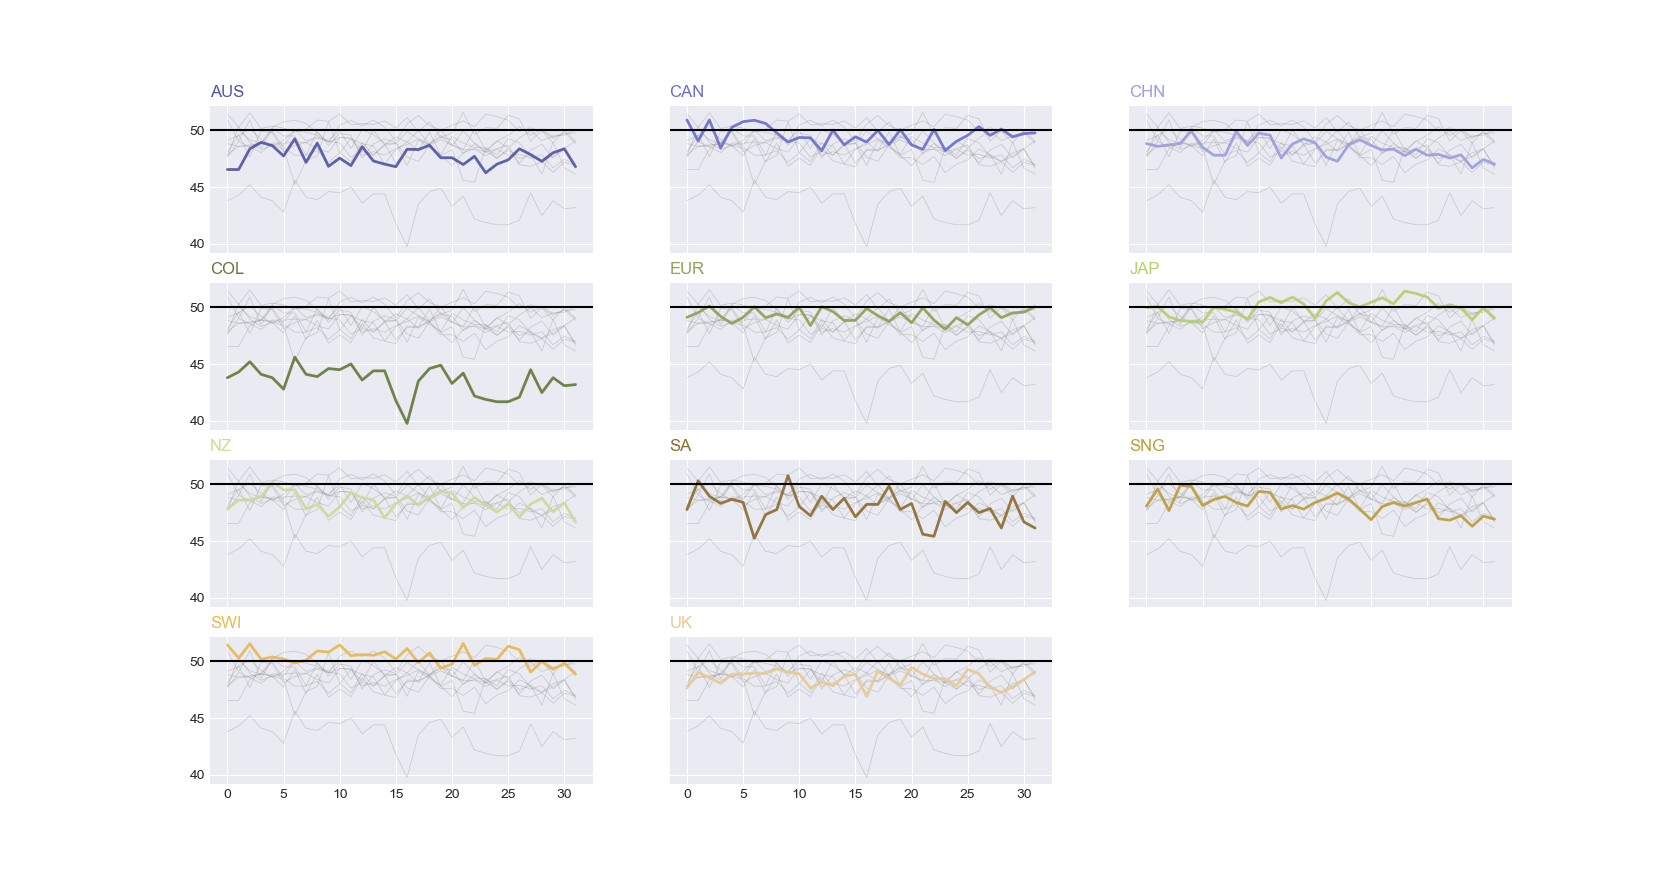
\includegraphics[scale = .8]{images/sentiment_analysis/manual_score.png}
        \caption{Accuracy Score of Tonality Dictionary Model at Varying Daily Intervals}
        \label{simulationfigure}
    \end{figure}
  \end{sidewaysfigure}

  \begin{sidewaysfigure}
    \begin{figure}[H]
        \centering
        \hspace*{-1.4in}
        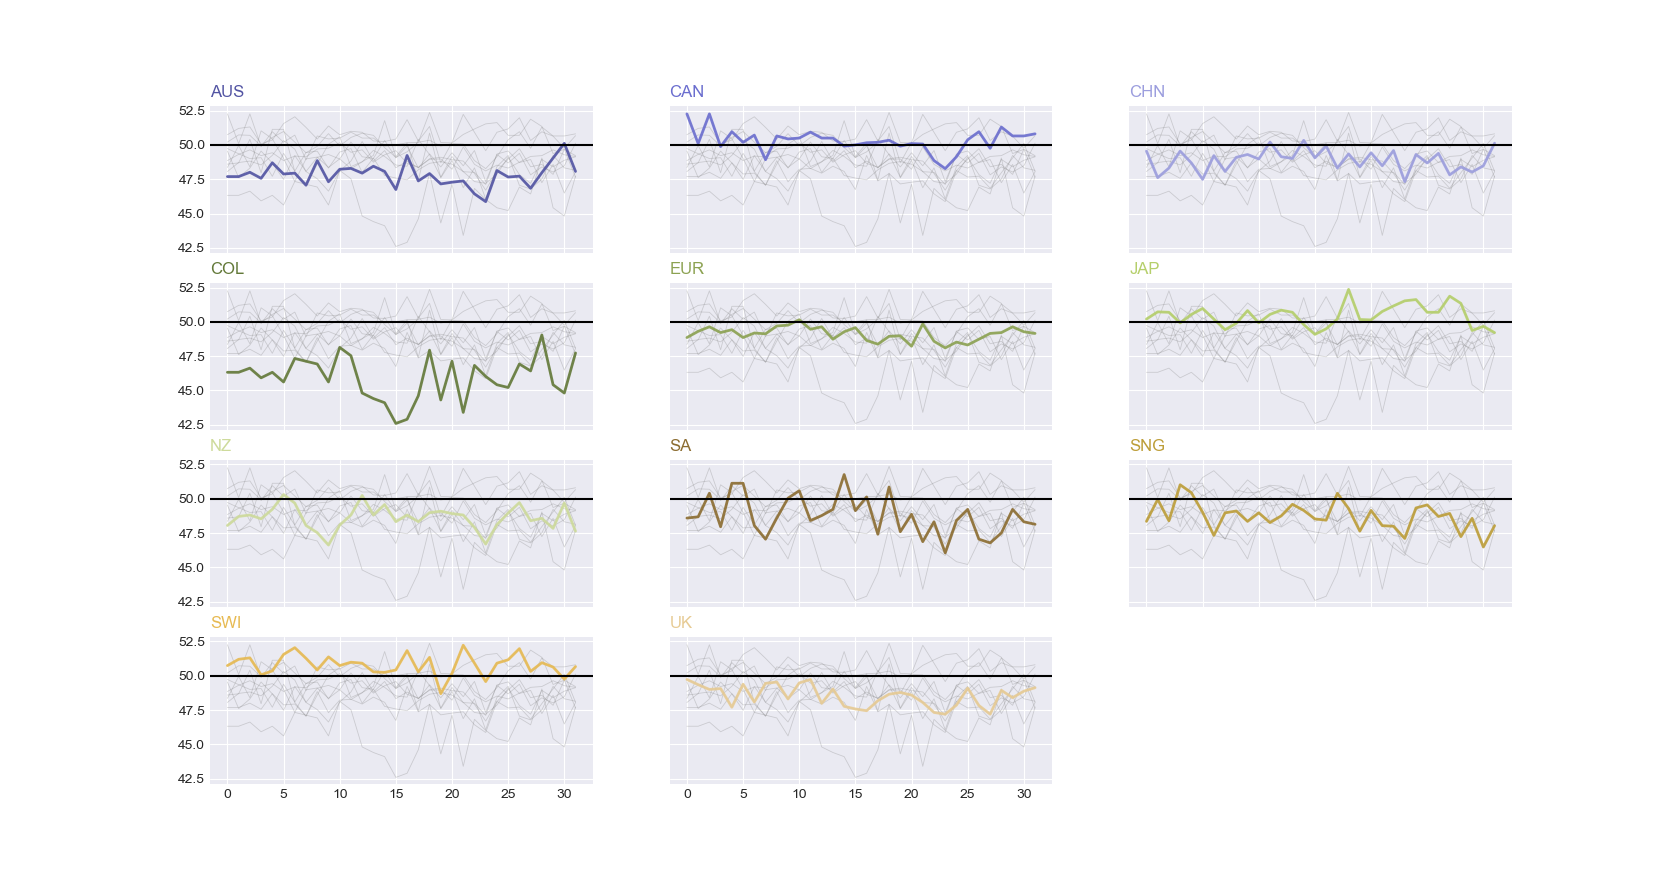
\includegraphics[scale = .8]{images/sentiment_analysis/vader_score.png}
        \caption{Accuracy Score of VADER Model at Varying Daily Intervals}
        \label{simulationfigure}
    \end{figure}
  \end{sidewaysfigure}

  \begin{sidewaysfigure}
    \begin{figure}[H]
        \centering
        \hspace*{-1.4in}
        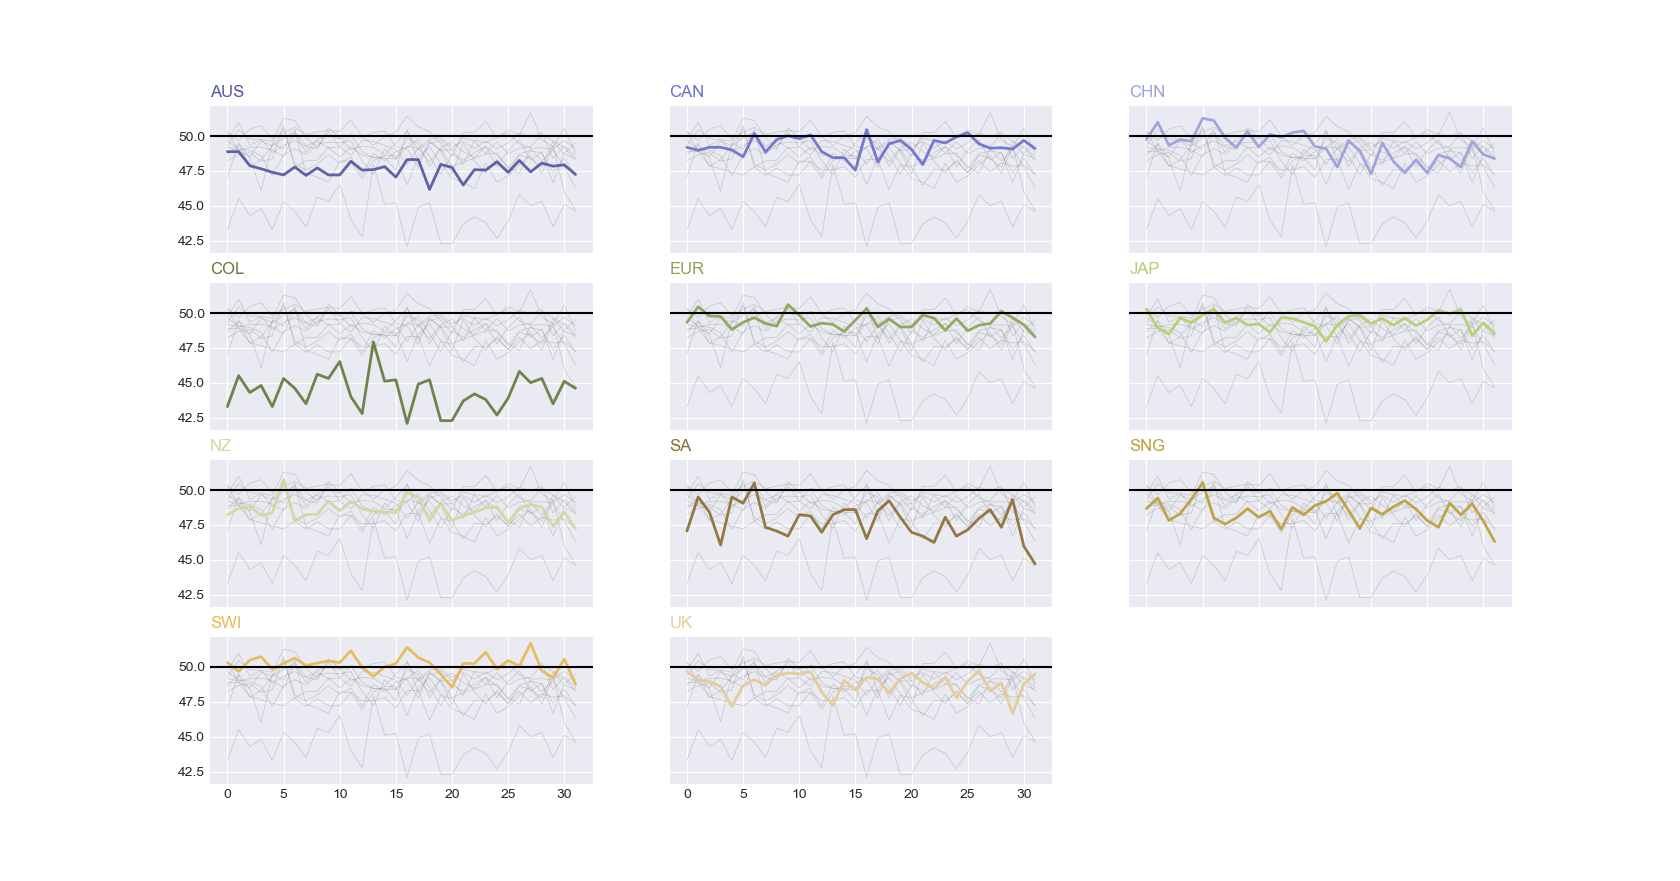
\includegraphics[scale = .8]{images/sentiment_analysis/textblob_score.png}
        \caption{Accuracy Score of TextBlob Model at Varying Daily Intervals}
        \label{simulationfigure}
    \end{figure}
  \end{sidewaysfigure}

  \begin{sidewaysfigure}
    \begin{figure}[H]
        \centering
        \hspace*{-1.4in}
        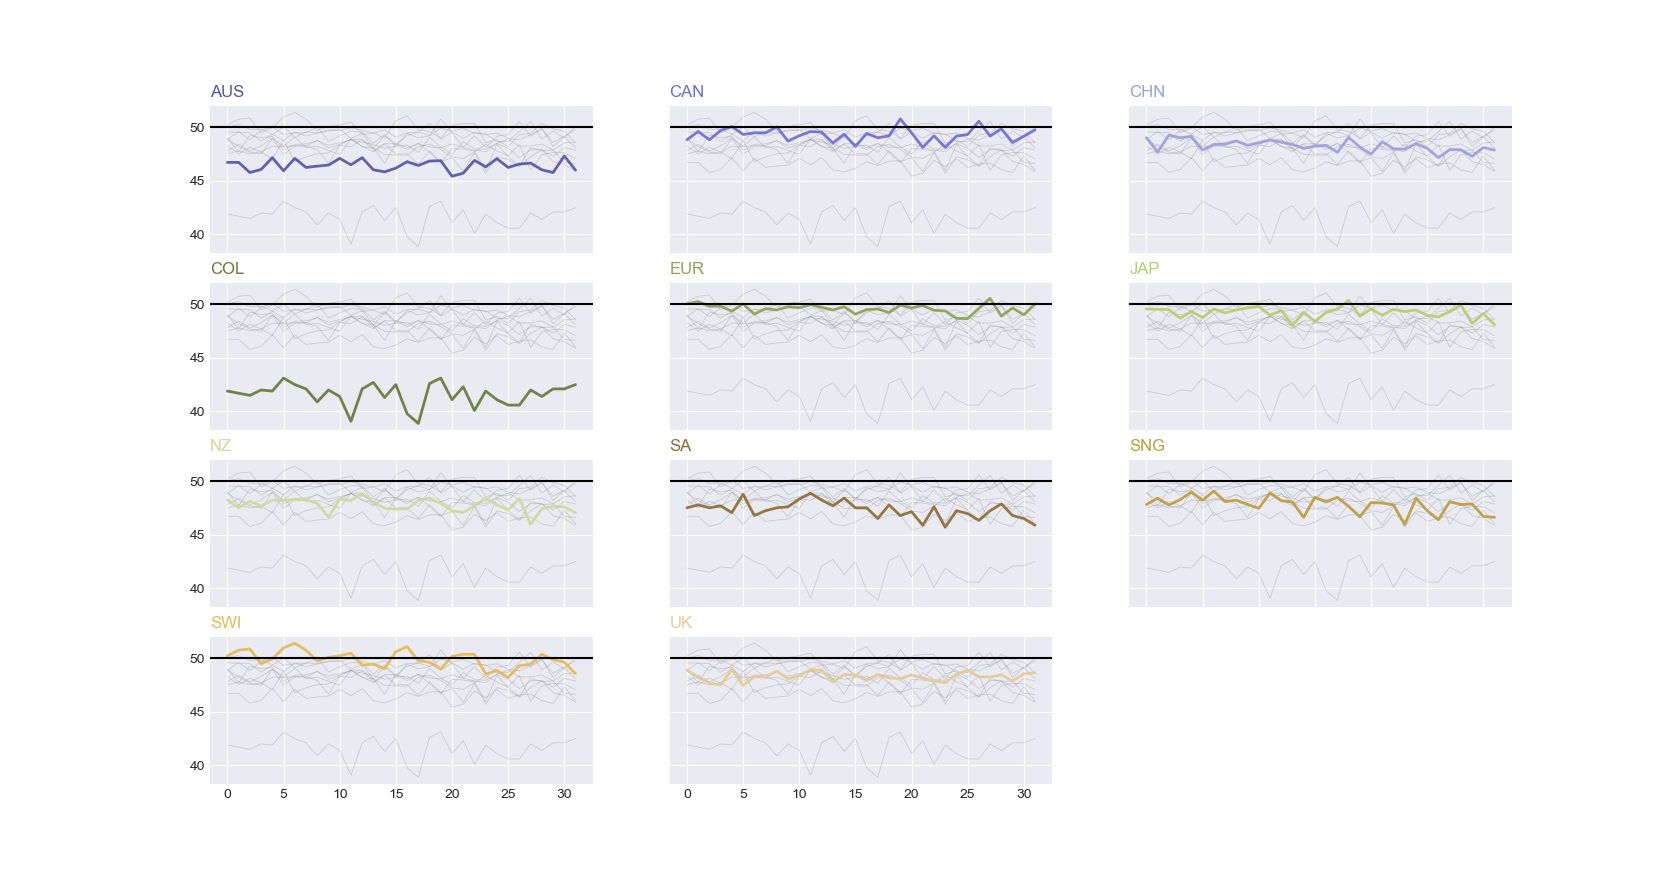
\includegraphics[scale = .8]{images/sentiment_analysis/hiv4_score.png}
        \caption{Accuracy Score of Harvard IV-4 Dictionary Model at Varying Daily Intervals}
        \label{simulationfigure}
    \end{figure}
  \end{sidewaysfigure}

  \begin{sidewaysfigure}
    \begin{figure}[H]
        \centering
        \hspace*{-1.4in}
        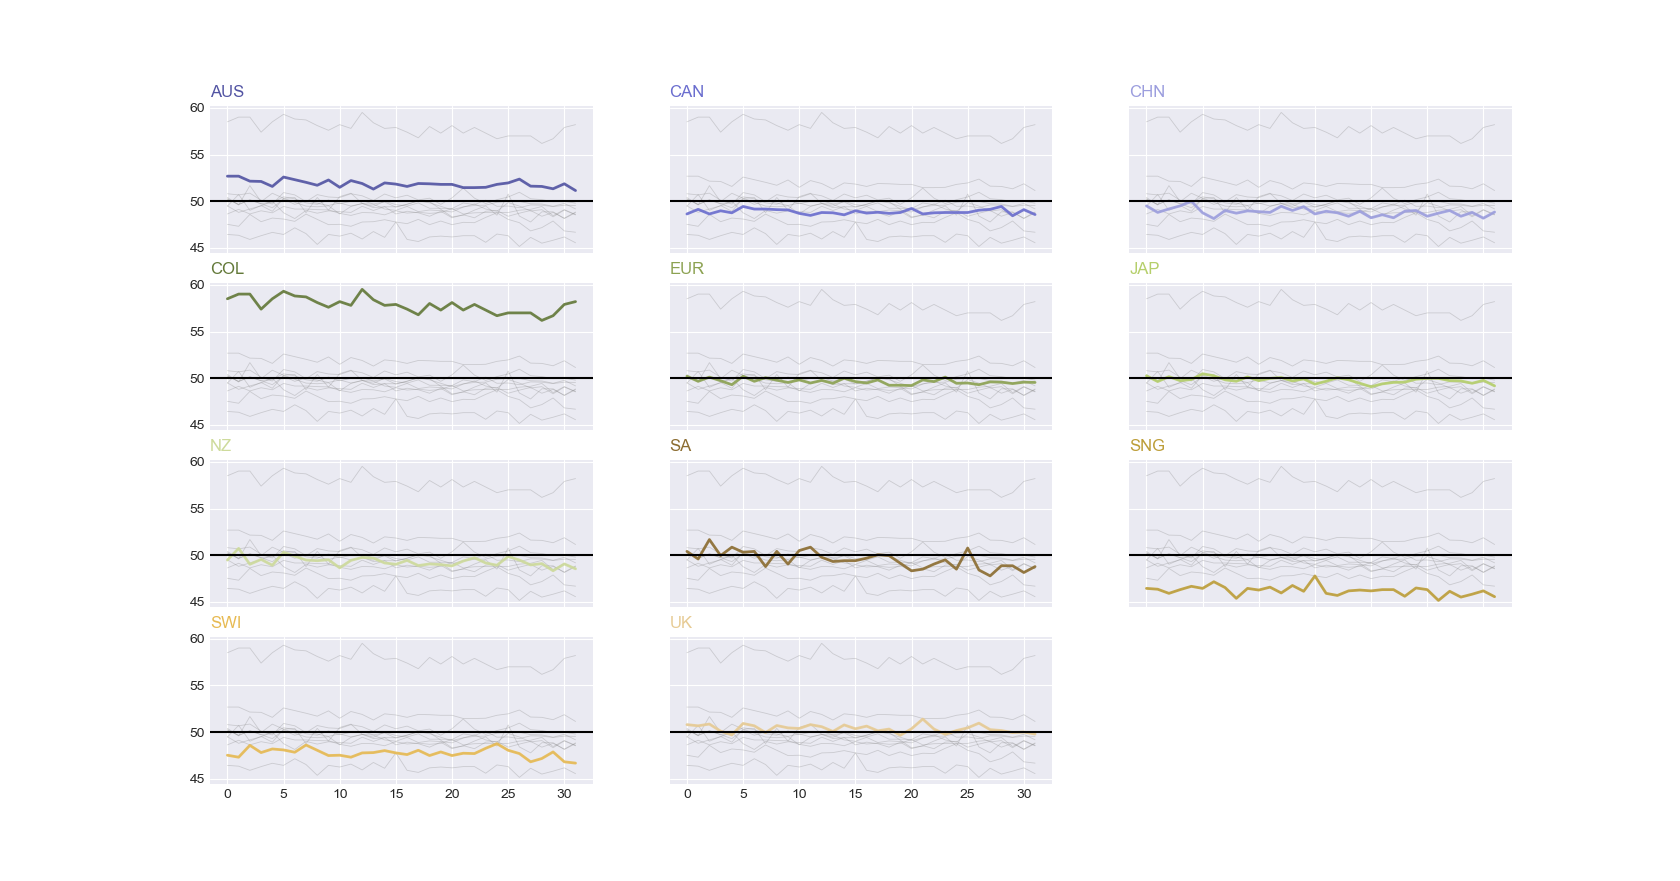
\includegraphics[scale = .8]{images/sentiment_analysis/lm_score.png}
        \caption{Accuracy Score of LM Dictionary Model at Varying Daily Intervals}
        \label{simulationfigure}
    \end{figure}
  \end{sidewaysfigure}

  \begin{sidewaysfigure}
    \begin{figure}[H]
        \centering
        \hspace*{-1.4in}
        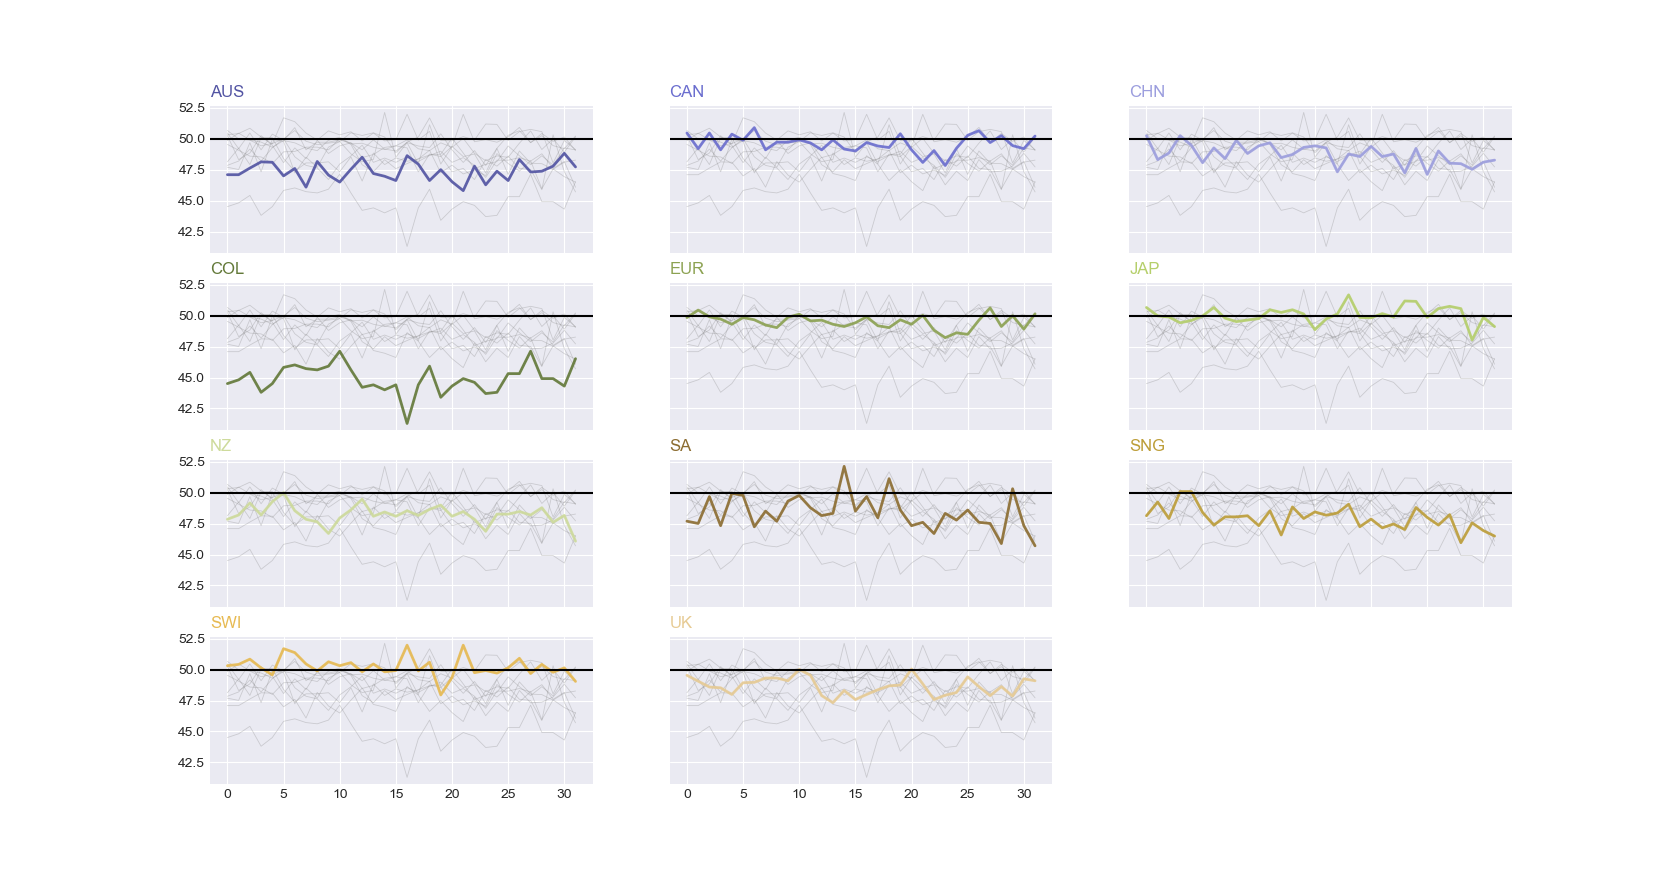
\includegraphics[scale = .8]{images/sentiment_analysis/aggregate_score.png}
        \caption{Accuracy Score of Aggregate Model at Varying Daily Intervals}
        \label{simulationfigure}
    \end{figure}
  \end{sidewaysfigure}

\newpage

The results of the sentiment model can also be viewed with the following app: \url{https://asaficontact.shinyapps.io/fx_sentiment/}. Different models seem to perform better for different countries. It is interesting to see how most of the models get their lowest accuracy score when trying to predict directional change in Colombia's exchange rate, while, the Loughran and Mcdonald dictionary model, on the other hand, appears to predict it with a high accuracy of about 60 percent. There seems to be no fixed relationship between the lagged interval for directional change in exchange rate and the accuracy score. Different country models seem to perform better at varying lagged intervals. For some countries, a model performs well at small lag values, while in case of others, the same model performs better at larger lag value.

\vspace*{4mm}

Combining sentiment scores of different models into one aggregate model does not seem to significantly improve our accuracy in predicting the directional change in exchange rates. The aggregate sentiment model assigns equal weights to all other models' tonality score when combining their results. This might cause the accurate model's prediction to be outweighed by the inaccurate ones if the number of models assigning an inaccurate sentiment score are greater than the ones assigning an accurate score. Using some form of dynamic weighting mechanism into the aggregate model might improve its accuracy.

\vspace*{4mm}

Different models seem to outperform the random walk model for different countries at varying lagged intervals. This means that their accuracy score for predicting directional change in foreign exchange rates is greater than 50\%. A random walk model, on an equally distributed dataset, has an accuracy score of 50\%. VADER seems to be the best performing sentiment model for all countries, while Harvard IV-4 Dictionary model and TextBlob seems to be the lowest accuracy models (failing to beat the random walk model in predicting directional change in exchange rate for most countries.)

\section{Discussion}

This chapter evaluates the importance of text preprocessing for developing an efficient sentiment analysis model. The results show that different sentiment models better predict the directional changes in exchange rates of different countries. This means that different sentiment models should be used for predicting different countries' directional change in exchange rates. For example, in case of Colombia, the Loughran and Mcdonald dictionary model appears to have the highest accuracy, while in case of Canada VADER seems to be the best performing one. This variation might be explained by the fact that the list of negative and positive words explaining a currency's market sentiment differs based on country. In our analysis of country specific word clouds, I find that the sorting by country mechanism, developed to classify news articles based on country, is not very efficient. This might be causing some country sentiment models to perform worse than the Random Walk model as misclassification of news articles can introduce noise in the dataset. Developing a more efficient sorting by country algorithm can further improve the predictive power of our sentiment analysis models in predicting directional change in exchange rates.

\chapter{Conclusion}

Grounded in macro-economic theory, this paper explores whether machine learning techniques can better predict the directional change in foreign exchange markets than the Random Walk model. I started off by analyzing Uncovered Interest Rate Parity (UIP) and how it fails to predict changes in exchange rates. Then, I used the interest rate of different countries to sort them into portfolios for carry trade. I also used supervised machine learning techniques such as Support Vector Machines (SVM) and Artificial Neural Networks (ANN) to predict the directional change in foreign exchange excess returns. Finally, I used Natural Language Processing (NLP) and Sentiment Analysis to create a variable for currency risk premium and market expectation that can be used to predict directional change in exchange rates.

\vspace*{4mm}

While testing for UIP, I found that it does not hold over the short and long run. A $\beta$ value of less than zero emphasizes the importance of currency risk premium in understanding the changes in exchange rates. It also shows the existence of arbitrage opportunity in the currency market. This means that traders can earn large profits over the short run by borrowing from low interest rate countries' bond market and investing in that of high interest rate countries'. I analyze the excess returns in carry trade market by creating a simulation based on historical interest rate and exchange rate data for trading on a monthly or semi-annual basis. According to the results, the returns on carry trade start to reduce with an increase in the trading interval. This means that a well diversified carry trade portfolio is more profitable over short trading intervals (daily or monthly) than longer trading intervals (semi-annual or annual).

\vspace*{4mm}

According to the spanning hypothesis, the yield curve, its expectation and term premium component span all relevant information related to the economic performance of a country. This means that we can understand the economic situation of a country by analyzing its bond market. Based on the spanning hypothesis, I use Principal Component Analysis (PCA) to extract the level, slope, and curvature of the yield curve and its components. Then, taking the resultant principal components, I use Support Vector Machines (SVM) and Artificial Neural Networks (ANN) to predict the directional change in foreign exchange excess returns. Compared to the SVMs, the ANNs more accurately predict the directional change in the exchange rate excess returns over the short run. This difference is attributed to the ability of Artificial Neural Networks to learn abstract features from raw data.

\vspace*{4mm}

Finally, in the last chapter, I use sentiment analysis to evaluate the tonality of foreign exchange news articles from investing.com to develop a variable for understanding currency risk premium and market expectations in order to predict the directional changes in the exchange rates. The foreign exchange markets are quite sensitive to unanticipated news and events. This means that we can develop a variable for understanding currency risk premium and market expectation by using sentiment analysis on financial news articles. In order to identify the model that most reliably captures the tonality of foreign exchange news articles, I use five different sentiment analysis models: Tonality model, VADER model, TextBlob model, Harvard IV-4 Dictionary model, and Loughran and Mcdonald Dictionary model. The results show that different sentiment models better predict the directional changes in exchange rates of different countries. For example, in case of Colombia, the Loughran and Mcdonald dictionary model appears to have the highest accuracy, while in case of Canada VADER seems to be the best performing one. Overall, the VADER sentiment model best captures the tonality of foreign exchange news articles for most countries in the dataset.

\vspace*{4mm}

All in all, this research finds evidence that machine learning models can more accurately predict directional change in exchange rates than the Random Walk model when the input features used to train the machine learning models are representative of the economic situation of a country. Hence, using macro-economic and financial theory to develop input features that capture the most relevant characteristics of a country’s economy can help us understand short run movements in the foreign exchange markets.

\bibliographystyle{apacite}
\bibliography{sources.bib}

\end{document}
